\documentclass[]{book}
\usepackage{lmodern}
\usepackage{amssymb,amsmath}
\usepackage{ifxetex,ifluatex}
\usepackage{fixltx2e} % provides \textsubscript
\ifnum 0\ifxetex 1\fi\ifluatex 1\fi=0 % if pdftex
  \usepackage[T1]{fontenc}
  \usepackage[utf8]{inputenc}
\else % if luatex or xelatex
  \ifxetex
    \usepackage{mathspec}
  \else
    \usepackage{fontspec}
  \fi
  \defaultfontfeatures{Ligatures=TeX,Scale=MatchLowercase}
\fi
% use upquote if available, for straight quotes in verbatim environments
\IfFileExists{upquote.sty}{\usepackage{upquote}}{}
% use microtype if available
\IfFileExists{microtype.sty}{%
\usepackage{microtype}
\UseMicrotypeSet[protrusion]{basicmath} % disable protrusion for tt fonts
}{}
\usepackage[margin=1in]{geometry}
\usepackage{hyperref}
\hypersetup{unicode=true,
            pdftitle={NIST/SEMATECH e-Handbook of Statistical Methods},
            pdfauthor={NIST},
            pdfborder={0 0 0},
            breaklinks=true}
\urlstyle{same}  % don't use monospace font for urls
\usepackage{natbib}
\bibliographystyle{apalike}
\usepackage{color}
\usepackage{fancyvrb}
\newcommand{\VerbBar}{|}
\newcommand{\VERB}{\Verb[commandchars=\\\{\}]}
\DefineVerbatimEnvironment{Highlighting}{Verbatim}{commandchars=\\\{\}}
% Add ',fontsize=\small' for more characters per line
\usepackage{framed}
\definecolor{shadecolor}{RGB}{248,248,248}
\newenvironment{Shaded}{\begin{snugshade}}{\end{snugshade}}
\newcommand{\KeywordTok}[1]{\textcolor[rgb]{0.13,0.29,0.53}{\textbf{#1}}}
\newcommand{\DataTypeTok}[1]{\textcolor[rgb]{0.13,0.29,0.53}{#1}}
\newcommand{\DecValTok}[1]{\textcolor[rgb]{0.00,0.00,0.81}{#1}}
\newcommand{\BaseNTok}[1]{\textcolor[rgb]{0.00,0.00,0.81}{#1}}
\newcommand{\FloatTok}[1]{\textcolor[rgb]{0.00,0.00,0.81}{#1}}
\newcommand{\ConstantTok}[1]{\textcolor[rgb]{0.00,0.00,0.00}{#1}}
\newcommand{\CharTok}[1]{\textcolor[rgb]{0.31,0.60,0.02}{#1}}
\newcommand{\SpecialCharTok}[1]{\textcolor[rgb]{0.00,0.00,0.00}{#1}}
\newcommand{\StringTok}[1]{\textcolor[rgb]{0.31,0.60,0.02}{#1}}
\newcommand{\VerbatimStringTok}[1]{\textcolor[rgb]{0.31,0.60,0.02}{#1}}
\newcommand{\SpecialStringTok}[1]{\textcolor[rgb]{0.31,0.60,0.02}{#1}}
\newcommand{\ImportTok}[1]{#1}
\newcommand{\CommentTok}[1]{\textcolor[rgb]{0.56,0.35,0.01}{\textit{#1}}}
\newcommand{\DocumentationTok}[1]{\textcolor[rgb]{0.56,0.35,0.01}{\textbf{\textit{#1}}}}
\newcommand{\AnnotationTok}[1]{\textcolor[rgb]{0.56,0.35,0.01}{\textbf{\textit{#1}}}}
\newcommand{\CommentVarTok}[1]{\textcolor[rgb]{0.56,0.35,0.01}{\textbf{\textit{#1}}}}
\newcommand{\OtherTok}[1]{\textcolor[rgb]{0.56,0.35,0.01}{#1}}
\newcommand{\FunctionTok}[1]{\textcolor[rgb]{0.00,0.00,0.00}{#1}}
\newcommand{\VariableTok}[1]{\textcolor[rgb]{0.00,0.00,0.00}{#1}}
\newcommand{\ControlFlowTok}[1]{\textcolor[rgb]{0.13,0.29,0.53}{\textbf{#1}}}
\newcommand{\OperatorTok}[1]{\textcolor[rgb]{0.81,0.36,0.00}{\textbf{#1}}}
\newcommand{\BuiltInTok}[1]{#1}
\newcommand{\ExtensionTok}[1]{#1}
\newcommand{\PreprocessorTok}[1]{\textcolor[rgb]{0.56,0.35,0.01}{\textit{#1}}}
\newcommand{\AttributeTok}[1]{\textcolor[rgb]{0.77,0.63,0.00}{#1}}
\newcommand{\RegionMarkerTok}[1]{#1}
\newcommand{\InformationTok}[1]{\textcolor[rgb]{0.56,0.35,0.01}{\textbf{\textit{#1}}}}
\newcommand{\WarningTok}[1]{\textcolor[rgb]{0.56,0.35,0.01}{\textbf{\textit{#1}}}}
\newcommand{\AlertTok}[1]{\textcolor[rgb]{0.94,0.16,0.16}{#1}}
\newcommand{\ErrorTok}[1]{\textcolor[rgb]{0.64,0.00,0.00}{\textbf{#1}}}
\newcommand{\NormalTok}[1]{#1}
\usepackage{longtable,booktabs}
\usepackage{graphicx,grffile}
\makeatletter
\def\maxwidth{\ifdim\Gin@nat@width>\linewidth\linewidth\else\Gin@nat@width\fi}
\def\maxheight{\ifdim\Gin@nat@height>\textheight\textheight\else\Gin@nat@height\fi}
\makeatother
% Scale images if necessary, so that they will not overflow the page
% margins by default, and it is still possible to overwrite the defaults
% using explicit options in \includegraphics[width, height, ...]{}
\setkeys{Gin}{width=\maxwidth,height=\maxheight,keepaspectratio}
\IfFileExists{parskip.sty}{%
\usepackage{parskip}
}{% else
\setlength{\parindent}{0pt}
\setlength{\parskip}{6pt plus 2pt minus 1pt}
}
\setlength{\emergencystretch}{3em}  % prevent overfull lines
\providecommand{\tightlist}{%
  \setlength{\itemsep}{0pt}\setlength{\parskip}{0pt}}
\setcounter{secnumdepth}{5}
% Redefines (sub)paragraphs to behave more like sections
\ifx\paragraph\undefined\else
\let\oldparagraph\paragraph
\renewcommand{\paragraph}[1]{\oldparagraph{#1}\mbox{}}
\fi
\ifx\subparagraph\undefined\else
\let\oldsubparagraph\subparagraph
\renewcommand{\subparagraph}[1]{\oldsubparagraph{#1}\mbox{}}
\fi

%%% Use protect on footnotes to avoid problems with footnotes in titles
\let\rmarkdownfootnote\footnote%
\def\footnote{\protect\rmarkdownfootnote}

%%% Change title format to be more compact
\usepackage{titling}

% Create subtitle command for use in maketitle
\newcommand{\subtitle}[1]{
  \posttitle{
    \begin{center}\large#1\end{center}
    }
}

\setlength{\droptitle}{-2em}
  \title{NIST/SEMATECH e-Handbook of Statistical Methods}
  \pretitle{\vspace{\droptitle}\centering\huge}
  \posttitle{\par}
  \author{NIST}
  \preauthor{\centering\large\emph}
  \postauthor{\par}
  \predate{\centering\large\emph}
  \postdate{\par}
  \date{2018-02-21}

\usepackage{booktabs}
\usepackage{amsthm}
\makeatletter
\def\thm@space@setup{%
  \thm@preskip=8pt plus 2pt minus 4pt
  \thm@postskip=\thm@preskip
}
\makeatother

\usepackage{amsthm}
\newtheorem{theorem}{Theorem}[chapter]
\newtheorem{lemma}{Lemma}[chapter]
\theoremstyle{definition}
\newtheorem{definition}{Definition}[chapter]
\newtheorem{corollary}{Corollary}[chapter]
\newtheorem{proposition}{Proposition}[chapter]
\theoremstyle{definition}
\newtheorem{example}{Example}[chapter]
\theoremstyle{definition}
\newtheorem{exercise}{Exercise}[chapter]
\theoremstyle{remark}
\newtheorem*{remark}{Remark}
\newtheorem*{solution}{Solution}
\begin{document}
\maketitle

{
\setcounter{tocdepth}{1}
\tableofcontents
}
\chapter*{Motivation}\label{motivation}
\addcontentsline{toc}{chapter}{Motivation}

This is a book redering the
\href{http://www.itl.nist.gov/div898/handbook/}{NISTNIST/SEMATECH
e-Handbook of Statistical Methods} in \emph{Markdown} and
\emph{tidyverse}.

The \textbf{bookdown} package can be installed from CRAN or Github:

\begin{Shaded}
\begin{Highlighting}[]
\KeywordTok{install.packages}\NormalTok{(}\StringTok{"bookdown"}\NormalTok{)}
\CommentTok{# or the development version}
\CommentTok{# devtools::install_github("rstudio/bookdown")}
\end{Highlighting}
\end{Shaded}

Remember each Rmd file contains one and only one chapter, and a chapter
is defined by the first-level heading \texttt{\#}.

To compile this example to PDF, you need XeLaTeX. You are recommended to
install TinyTeX (which includes XeLaTeX):
\url{https://yihui.name/tinytex/}.

\chapter{Exploratory Data Analysis}\label{exploratory-data-analysis}

\section{EDA Introduction}\label{eda-introduction}

\subsection{What is EDA?}\label{what-is-eda}

\subsubsection{Approach}\label{approach}

Exploratory Data Analysis (EDA) is an approach/philosophy for data
analysis that employs a variety of techniques (mostly graphical) to

\begin{itemize}
\tightlist
\item
  maximize insight into a data set;
\item
  uncover underlying structure;
\item
  extract important variables;
\item
  detect outliers and anomalies;
\item
  test underlying assumptions;
\item
  develop parsimonious models; and
\item
  determine optimal factor settings.
\end{itemize}

Focus The EDA approach is precisely that--an approach--not a set of
techniques, but an attitude/philosophy about how a data analysis should
be carried out.

\subsubsection{Philosophy}\label{philosophy}

EDA is not identical to statistical graphics although the two terms are
used almost interchangeably. Statistical graphics is a collection of
techniques--all graphically based and all focusing on one data
characterization aspect. EDA encompasses a larger venue; EDA is an
approach to data analysis that postpones the usual assumptions about
what kind of model the data follow with the more direct approach of
allowing the data itself to reveal its underlying structure and model.
EDA is not a mere collection of techniques; EDA is a philosophy as to
how we dissect a data set; what we look for; how we look; and how we
interpret. It is true that EDA heavily uses the collection of techniques
that we call ``statistical graphics'', but it is not identical to
statistical graphics per se.

\subsubsection{History}\label{history}

The seminal work in EDA is Exploratory Data Analysis, Tukey, (1977).
Over the years it has benefitted from other noteworthy publications such
as Data Analysis and Regression, Mosteller and Tukey (1977), Interactive
Data Analysis, Hoaglin (1977), The ABC's of EDA, Velleman and Hoaglin
(1981) and has gained a large following as ``the'' way to analyze a data
set.

\subsubsection{Techniques}\label{techniques}

Most EDA techniques are graphical in nature with a few quantitative
techniques. The reason for the heavy reliance on graphics is that by its
very nature the main role of EDA is to open-mindedly explore, and
graphics gives the analysts unparalleled power to do so, enticing the
data to reveal its structural secrets, and being always ready to gain
some new, often unsuspected, insight into the data. In combination with
the natural pattern-recognition capabilities that we all possess,
graphics provides, of course, unparalleled power to carry this out. The
particular graphical techniques employed in EDA are often quite simple,
consisting of various techniques of:

\begin{itemize}
\tightlist
\item
  Plotting the raw data (such as data traces, histograms, bihistograms,
  probability plots, lag plots, block plots, and Youden plots.
\item
  Plotting simple statistics such as mean plots, standard deviation
  plots, box plots, and main effects plots of the raw data.
\item
  Positioning such plots so as to maximize our natural
  pattern-recognition abilities, such as using multiple plots per page.
\end{itemize}

\subsection{EDA versus Classical and
Bayesian}\label{eda-versus-classical-and-bayesian}

How Does Exploratory Data Analysis differ from Classical Data Analysis?

\subsubsection{Data Analysis Approaches}\label{data-analysis-approaches}

EDA is a data analysis approach. What other data analysis approaches
exist and how does EDA differ from these other approaches? Three popular
data analysis approaches are:

\begin{itemize}
\tightlist
\item
  Classical
\item
  Exploratory (EDA)
\item
  Bayesian
\end{itemize}

\subsubsection{Paradigms for Analysis
Techniques}\label{paradigms-for-analysis-techniques}

These three approaches are similar in that they all start with a general
science/engineering problem and all yield science/engineering
conclusions. The difference is the sequence and focus of the
intermediate steps.

\begin{itemize}
\tightlist
\item
  For classical analysis, the sequence is Problem =\textgreater{} Data
  =\textgreater{} Model =\textgreater{} Analysis =\textgreater{}
  Conclusions
\item
  For EDA, the sequence is Problem =\textgreater{} Data =\textgreater{}
  Analysis =\textgreater{} Model =\textgreater{} Conclusions
\item
  For Bayesian, the sequence is Problem =\textgreater{} Data
  =\textgreater{} Model =\textgreater{} Prior Distribution
  =\textgreater{} Analysis =\textgreater{} Conclusions
\end{itemize}

\subsubsection{Method of dealing with underlying model for the data
distinguishes the 3
approaches}\label{method-of-dealing-with-underlying-model-for-the-data-distinguishes-the-3-approaches}

Thus for classical analysis, the data collection is followed by the
imposition of a model (normality, linearity, etc.) and the analysis,
estimation, and testing that follows are focused on the parameters of
that model. For EDA, the data collection is not followed by a model
imposition; rather it is followed immediately by analysis with a goal of
inferring what model would be appropriate. Finally, for a Bayesian
analysis, the analyst attempts to incorporate scientific/engineering
knowledge/expertise into the analysis by imposing a data-independent
distribution on the parameters of the selected model; the analysis thus
consists of formally combining both the prior distribution on the
parameters and the collected data to jointly make inferences and/or test
assumptions about the model parameters. In the real world, data analysts
freely mix elements of all of the above three approaches (and other
approaches). The above distinctions were made to emphasize the major
differences among the three approaches.

\subsubsection{Further discussion of the distinction between the
classical and EDA
approaches}\label{further-discussion-of-the-distinction-between-the-classical-and-eda-approaches}

Focusing on EDA versus classical, these two approaches differ as
follows:

\begin{longtable}[]{@{}lll@{}}
\toprule
\begin{minipage}[b]{0.14\columnwidth}\raggedright\strut
Approacches\strut
\end{minipage} & \begin{minipage}[b]{0.39\columnwidth}\raggedright\strut
Classicial\strut
\end{minipage} & \begin{minipage}[b]{0.39\columnwidth}\raggedright\strut
EDA\strut
\end{minipage}\tabularnewline
\midrule
\endhead
\begin{minipage}[t]{0.14\columnwidth}\raggedright\strut
Models\strut
\end{minipage} & \begin{minipage}[t]{0.39\columnwidth}\raggedright\strut
The classical approach imposes models (both deterministic and
probabilistic) on the data. Deterministic models include, for example,
regression models and analysis of variance (ANOVA) models. The most
common probabilistic model assumes that the errors about the
deterministic model are normally distributed--this assumption affects
the validity of the ANOVA F tests.\strut
\end{minipage} & \begin{minipage}[t]{0.39\columnwidth}\raggedright\strut
The Exploratory Data Analysis approach does not impose deterministic or
probabilistic models on the data. On the contrary, the EDA approach
allows the data to suggest admissible models that best fit the
data.\strut
\end{minipage}\tabularnewline
\begin{minipage}[t]{0.14\columnwidth}\raggedright\strut
Focus\strut
\end{minipage} & \begin{minipage}[t]{0.39\columnwidth}\raggedright\strut
The two approaches differ substantially in focus. For classical
analysis, the focus is on the model--estimating parameters of the model
and generating predicted values from the model.\strut
\end{minipage} & \begin{minipage}[t]{0.39\columnwidth}\raggedright\strut
For exploratory data analysis, the focus is on the data--its structure,
outliers, and models suggested by the data.\strut
\end{minipage}\tabularnewline
\begin{minipage}[t]{0.14\columnwidth}\raggedright\strut
Techniques\strut
\end{minipage} & \begin{minipage}[t]{0.39\columnwidth}\raggedright\strut
Classical techniques are generally quantitative in nature. They include
ANOVA, t tests, chi-squared tests, and F tests.\strut
\end{minipage} & \begin{minipage}[t]{0.39\columnwidth}\raggedright\strut
Exploratory EDA techniques are generally graphical. They include scatter
plots, character plots, box plots, histograms, bihistograms, probability
plots, residual plots, and mean plots.\strut
\end{minipage}\tabularnewline
\begin{minipage}[t]{0.14\columnwidth}\raggedright\strut
Rigor\strut
\end{minipage} & \begin{minipage}[t]{0.39\columnwidth}\raggedright\strut
Classical techniques serve as the probabilistic foundation of science
and engineering; the most important characteristic of classical
techniques is that they are rigorous, formal, and ``objective''.\strut
\end{minipage} & \begin{minipage}[t]{0.39\columnwidth}\raggedright\strut
EDA techniques do not share in that rigor or formality. EDA techniques
make up for that lack of rigor by being very suggestive, indicative, and
insightful about what the appropriate model should be. EDA techniques
are subjective and depend on interpretation which may differ from
analyst to analyst, although experienced analysts commonly arrive at
identical conclusions.\strut
\end{minipage}\tabularnewline
\begin{minipage}[t]{0.14\columnwidth}\raggedright\strut
Data Treatment\strut
\end{minipage} & \begin{minipage}[t]{0.39\columnwidth}\raggedright\strut
Classical estimation techniques have the characteristic of taking all of
the data and mapping the data into a few numbers (``estimates''). This
is both a virtue and a vice. The virtue is that these few numbers focus
on important characteristics (location, variation, etc.) of the
population. The vice is that concentrating on these few characteristics
can filter out other characteristics (skewness, tail length,
autocorrelation, etc.) of the same population. In this sense there is a
loss of information due to this ``filtering'' process.\strut
\end{minipage} & \begin{minipage}[t]{0.39\columnwidth}\raggedright\strut
The EDA approach, on the other hand, often makes use of (and shows) all
of the available data. In this sense there is no corresponding loss of
information.\strut
\end{minipage}\tabularnewline
\begin{minipage}[t]{0.14\columnwidth}\raggedright\strut
Assumptions\strut
\end{minipage} & \begin{minipage}[t]{0.39\columnwidth}\raggedright\strut
The ``good news'' of the classical approach is that tests based on
classical techniques are usually very sensitive--that is, if a true
shift in location, say, has occurred, such tests frequently have the
power to detect such a shift and to conclude that such a shift is
``statistically significant''. The ``bad news'' is that classical tests
depend on underlying assumptions (e.g., normality), and hence the
validity of the test conclusions becomes dependent on the validity of
the underlying assumptions. Worse yet, the exact underlying assumptions
may be unknown to the analyst, or if known, untested. Thus the validity
of the scientific conclusions becomes intrinsically linked to the
validity of the underlying assumptions. In practice, if such assumptions
are unknown or untested, the validity of the scientific conclusions
becomes suspect.\strut
\end{minipage} & \begin{minipage}[t]{0.39\columnwidth}\raggedright\strut
Many EDA techniques make little or no assumptions--they present and show
the data--all of the data--as is, with fewer encumbering
assumptions.\strut
\end{minipage}\tabularnewline
\bottomrule
\end{longtable}

\subsection{EDA vs.~Summary}\label{eda-vs.summary}

How Does Exploratory Data Analysis Differ from Summary Analysis?

\subsubsection{Summary}\label{summary}

A summary analysis is simply a numeric reduction of a historical data
set. It is quite passive. Its focus is in the past. Quite commonly, its
purpose is to simply arrive at a few key statistics (for example, mean
and standard deviation) which may then either replace the data set or be
added to the data set in the form of a summary table.

\subsubsection{Exploratory}\label{exploratory}

In contrast, EDA has as its broadest goal the desire to gain insight
into the engineering/scientific process behind the data. Whereas summary
statistics are passive and historical, EDA is active and futuristic. In
an attempt to ``understand'' the process and improve it in the future,
EDA uses the data as a ``window'' to peer into the heart of the process
that generated the data. There is an archival role in the research and
manufacturing world for summary statistics, but there is an enormously
larger role for the EDA approach.

\subsection{What are the EDA Goals?}\label{what-are-the-eda-goals}

\subsubsection{Primary and Secondary
Goals}\label{primary-and-secondary-goals}

The primary goal of EDA is to maximize the analyst's insight into a data
set and into the underlying structure of a data set, while providing all
of the specific items that an analyst would want to extract from a data
set, such as:

\begin{itemize}
\tightlist
\item
  a good-fitting, parsimonious model
\item
  a list of outliers
\item
  a sense of robustness of conclusions
\item
  estimates for parameters
\item
  uncertainties for those estimates
\item
  a ranked list of important factors
\item
  conclusions as to whether individual factors are statistically
  significant
\item
  optimal settings
\end{itemize}

\subsubsection{Insight into the Data}\label{insight-into-the-data}

Insight implies detecting and uncovering underlying structure in the
data. Such underlying structure may not be encapsulated in the list of
items above; such items serve as the specific targets of an analysis,
but the real insight and ``feel'' for a data set comes as the analyst
judiciously probes and explores the various subtleties of the data. The
``feel'' for the data comes almost exclusively from the application of
various graphical techniques, the collection of which serves as the
window into the essence of the data. Graphics are irreplaceable--there
are no quantitative analogues that will give the same insight as
well-chosen graphics. To get a ``feel'' for the data, it is not enough
for the analyst to know what is in the data; the analyst also must know
what is not in the data, and the only way to do that is to draw on our
own human pattern-recognition and comparative abilities in the context
of a series of judicious graphical techniques applied to the data.

\subsection{The Role of Graphics}\label{the-role-of-graphics}

\subsubsection{Quantitative/Graphical}\label{quantitativegraphical}

Statistics and data analysis procedures can broadly be split into two
parts:

\begin{itemize}
\tightlist
\item
  quantitative
\item
  graphical
\end{itemize}

\paragraph{Quantitative}\label{quantitative}

Quantitative techniques are the set of statistical procedures that yield
numeric or tabular output. Examples of quantitative techniques include:

\begin{itemize}
\item
  hypothesis testing
\item
  analysis of variance
\item
  point estimates and confidence intervals
\item
  least squares regression These and similar techniques are all valuable
  and are mainstream in terms of classical analysis. Graphical On the
  other hand, there is a large collection of statistical tools that we
  generally refer to as graphical techniques. These include:
\item
  scatter plots
\item
  histograms
\item
  probability plots
\item
  residual plots
\item
  box plots
\item
  block plots
\end{itemize}

\subsubsection{EDA Approach Relies Heavily on Graphical
Techniques}\label{eda-approach-relies-heavily-on-graphical-techniques}

The EDA approach relies heavily on these and similar graphical
techniques. Graphical procedures are not just tools that we could use in
an EDA context, they are tools that we must use. Such graphical tools
are the shortest path to gaining insight into a data set in terms of

\begin{itemize}
\tightlist
\item
  testing assumptions
\item
  model selection
\item
  model validation
\item
  estimator selection
\item
  relationship identification
\item
  factor effect determination
\item
  outlier detection
\end{itemize}

If one is not using statistical graphics, then one is forfeiting insight
into one or more aspects of the underlying structure of the data.

\subsection{An EDA/Graphics Example}\label{an-edagraphics-example}

\subsubsection{Anscombe Example}\label{anscombe-example}

A simple, classic (Anscombe) example of the central role that graphics
play in terms of providing insight into a data set starts with the
following data set: Data\\
X Y 10.00 8.04 8.00 6.95 13.00 7.58 9.00 8.81 11.00 8.33 14.00 9.96 6.00
7.24 4.00 4.26 12.00 10.84 7.00 4.82 5.00 5.68

\begin{Shaded}
\begin{Highlighting}[]
\KeywordTok{print}\NormalTok{(anscombe[}\KeywordTok{c}\NormalTok{(}\StringTok{"x1"}\NormalTok{,}\StringTok{"y1"}\NormalTok{)])}
\end{Highlighting}
\end{Shaded}

\begin{verbatim}
##    x1    y1
## 1  10  8.04
## 2   8  6.95
## 3  13  7.58
## 4   9  8.81
## 5  11  8.33
## 6  14  9.96
## 7   6  7.24
## 8   4  4.26
## 9  12 10.84
## 10  7  4.82
## 11  5  5.68
\end{verbatim}

\subsubsection{Summary Statistics}\label{summary-statistics}

If the goal of the analysis is to compute summary statistics plus
determine the best linear fit for Y as a function of X, the results
might be given as: \textgreater{} N = 11 \textgreater{} Mean of X = 9.0
\textgreater{} Mean of Y = 7.5 \textgreater{} Intercept = 3
\textgreater{} Slope = 0.5 \textgreater{} Residual standard deviation =
1.237 \textgreater{} Correlation = 0.816

\begin{Shaded}
\begin{Highlighting}[]
\KeywordTok{print}\NormalTok{(skimr}\OperatorTok{::}\KeywordTok{skim}\NormalTok{(anscombe[}\KeywordTok{c}\NormalTok{(}\StringTok{"x1"}\NormalTok{, }\StringTok{"y1"}\NormalTok{)]))}
\end{Highlighting}
\end{Shaded}

\begin{verbatim}
## Skim summary statistics
##  n obs: 11 
##  n variables: 2 
## 
## Variable type: numeric 
##  variable missing complete  n mean   sd   p0  p25 median   p75  p100
##        x1       0       11 11  9   3.32 4    6.5    9    11.5  14   
##        y1       0       11 11  7.5 2.03 4.26 6.31   7.58  8.57 10.84
##      hist
##  ▇▃▃▇▃▃▃▇
##  ▅▂▁▅▇▂▂▂
\end{verbatim}

\begin{Shaded}
\begin{Highlighting}[]
\KeywordTok{print}\NormalTok{(}\KeywordTok{summary}\NormalTok{(}\KeywordTok{lm}\NormalTok{(y1}\OperatorTok{~}\NormalTok{x1, }\DataTypeTok{data =}\NormalTok{ anscombe)))}
\end{Highlighting}
\end{Shaded}

\begin{verbatim}
## 
## Call:
## lm(formula = y1 ~ x1, data = anscombe)
## 
## Residuals:
##      Min       1Q   Median       3Q      Max 
## -1.92127 -0.45577 -0.04136  0.70941  1.83882 
## 
## Coefficients:
##             Estimate Std. Error t value Pr(>|t|)   
## (Intercept)   3.0001     1.1247   2.667  0.02573 * 
## x1            0.5001     0.1179   4.241  0.00217 **
## ---
## Signif. codes:  0 '***' 0.001 '**' 0.01 '*' 0.05 '.' 0.1 ' ' 1
## 
## Residual standard error: 1.237 on 9 degrees of freedom
## Multiple R-squared:  0.6665, Adjusted R-squared:  0.6295 
## F-statistic: 17.99 on 1 and 9 DF,  p-value: 0.00217
\end{verbatim}

The above quantitative analysis, although valuable, gives us only
limited insight into the data.

\subsubsection{Scatter Plot}\label{scatter-plot}

n contrast, the following simple scatter plot of the data

\begin{Shaded}
\begin{Highlighting}[]
\KeywordTok{ggplot}\NormalTok{(anscombe, }\KeywordTok{aes}\NormalTok{(x1, y1)) }\OperatorTok{+}\StringTok{ }\KeywordTok{geom_point}\NormalTok{() }\OperatorTok{+}\StringTok{ }\KeywordTok{geom_smooth}\NormalTok{(}\DataTypeTok{method =} \StringTok{"lm"}\NormalTok{)}
\end{Highlighting}
\end{Shaded}

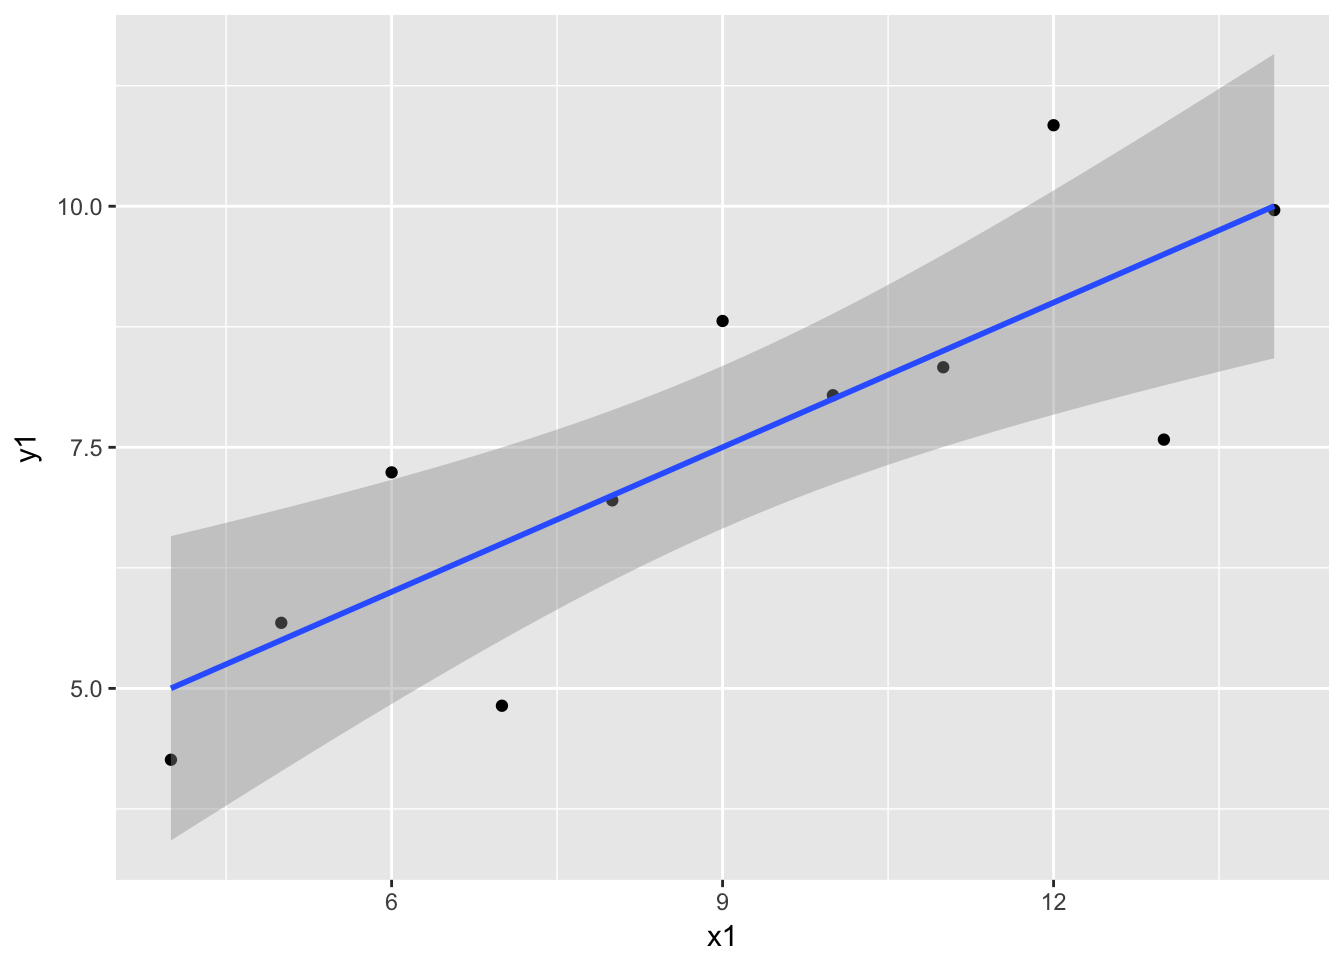
\includegraphics{eda_files/figure-latex/unnamed-chunk-5-1.pdf}

A scatter plot of the Anscombe data suggests the following:

\begin{itemize}
\tightlist
\item
  The data set ``behaves like'' a linear curve with some scatter;
\item
  there is no justification for a more complicated model (e.g.,
  quadratic);
\item
  there are no outliers;
\item
  the vertical spread of the data appears to be of equal height
  irrespective of the X-value; this indicates that the data are
  equally-precise throughout and so a ``regular'' (that is,
  equi-weighted) fit is appropriate.
\end{itemize}

\subsubsection{Three Additional Data
Sets}\label{three-additional-data-sets}

This kind of characterization for the data serves as the core for
getting insight/feel for the data. Such insight/feel does not come from
the quantitative statistics; on the contrary, calculations of
quantitative statistics such as intercept and slope should be subsequent
to the characterization and will make sense only if the characterization
is true. To illustrate the loss of information that results when the
graphics insight step is skipped, consider the following three data sets
{[}Anscombe data sets 2, 3, and 4{]}: X2 Y2 X3 Y3 X4 Y4 10.00 9.14 10.00
7.46 8.00 6.58 8.00 8.14 8.00 6.77 8.00 5.76 13.00 8.74 13.00 12.74 8.00
7.71 9.00 8.77 9.00 7.11 8.00 8.84 11.00 9.26 11.00 7.81 8.00 8.47 14.00
8.10 14.00 8.84 8.00 7.04 6.00 6.13 6.00 6.08 8.00 5.25 4.00 3.10 4.00
5.39 19.00 12.50 12.00 9.13 12.00 8.15 8.00 5.56 7.00 7.26 7.00 6.42
8.00 7.91 5.00 4.74 5.00 5.73 8.00 6.89

\begin{Shaded}
\begin{Highlighting}[]
\KeywordTok{print}\NormalTok{(skimr}\OperatorTok{::}\KeywordTok{skim}\NormalTok{(anscombe[}\KeywordTok{c}\NormalTok{(}\StringTok{"x2"}\NormalTok{, }\StringTok{"y2"}\NormalTok{, }\StringTok{"x3"}\NormalTok{, }\StringTok{"y3"}\NormalTok{, }\StringTok{"x4"}\NormalTok{, }\StringTok{"y4"}\NormalTok{)]))}
\end{Highlighting}
\end{Shaded}

\begin{verbatim}
## Skim summary statistics
##  n obs: 11 
##  n variables: 6 
## 
## Variable type: numeric 
##  variable missing complete  n mean   sd   p0  p25 median   p75  p100
##        x2       0       11 11  9   3.32 4    6.5    9    11.5  14   
##        x3       0       11 11  9   3.32 4    6.5    9    11.5  14   
##        x4       0       11 11  9   3.32 8    8      8     8    19   
##        y2       0       11 11  7.5 2.03 3.1  6.7    8.14  8.95  9.26
##        y3       0       11 11  7.5 2.03 5.39 6.25   7.11  7.98 12.74
##        y4       0       11 11  7.5 2.03 5.25 6.17   7.04  8.19 12.5 
##      hist
##  ▇▃▃▇▃▃▃▇
##  ▇▃▃▇▃▃▃▇
##  ▇▁▁▁▁▁▁▁
##  ▂▁▂▂▁▂▃▇
##  ▇▇▅▅▁▁▁▂
##  ▇▇▅▅▁▁▁▂
\end{verbatim}

\begin{Shaded}
\begin{Highlighting}[]
\KeywordTok{print}\NormalTok{(}\KeywordTok{summary}\NormalTok{(}\KeywordTok{lm}\NormalTok{(y1}\OperatorTok{~}\NormalTok{x1, }\DataTypeTok{data =}\NormalTok{ anscombe)))}
\end{Highlighting}
\end{Shaded}

\begin{verbatim}
## 
## Call:
## lm(formula = y1 ~ x1, data = anscombe)
## 
## Residuals:
##      Min       1Q   Median       3Q      Max 
## -1.92127 -0.45577 -0.04136  0.70941  1.83882 
## 
## Coefficients:
##             Estimate Std. Error t value Pr(>|t|)   
## (Intercept)   3.0001     1.1247   2.667  0.02573 * 
## x1            0.5001     0.1179   4.241  0.00217 **
## ---
## Signif. codes:  0 '***' 0.001 '**' 0.01 '*' 0.05 '.' 0.1 ' ' 1
## 
## Residual standard error: 1.237 on 9 degrees of freedom
## Multiple R-squared:  0.6665, Adjusted R-squared:  0.6295 
## F-statistic: 17.99 on 1 and 9 DF,  p-value: 0.00217
\end{verbatim}

\begin{Shaded}
\begin{Highlighting}[]
\KeywordTok{print}\NormalTok{(}\KeywordTok{summary}\NormalTok{(}\KeywordTok{lm}\NormalTok{(y1}\OperatorTok{~}\NormalTok{x1, }\DataTypeTok{data =}\NormalTok{ anscombe)))}
\end{Highlighting}
\end{Shaded}

\begin{verbatim}
## 
## Call:
## lm(formula = y1 ~ x1, data = anscombe)
## 
## Residuals:
##      Min       1Q   Median       3Q      Max 
## -1.92127 -0.45577 -0.04136  0.70941  1.83882 
## 
## Coefficients:
##             Estimate Std. Error t value Pr(>|t|)   
## (Intercept)   3.0001     1.1247   2.667  0.02573 * 
## x1            0.5001     0.1179   4.241  0.00217 **
## ---
## Signif. codes:  0 '***' 0.001 '**' 0.01 '*' 0.05 '.' 0.1 ' ' 1
## 
## Residual standard error: 1.237 on 9 degrees of freedom
## Multiple R-squared:  0.6665, Adjusted R-squared:  0.6295 
## F-statistic: 17.99 on 1 and 9 DF,  p-value: 0.00217
\end{verbatim}

\begin{Shaded}
\begin{Highlighting}[]
\KeywordTok{print}\NormalTok{(}\KeywordTok{summary}\NormalTok{(}\KeywordTok{lm}\NormalTok{(y1}\OperatorTok{~}\NormalTok{x1, }\DataTypeTok{data =}\NormalTok{ anscombe)))}
\end{Highlighting}
\end{Shaded}

\begin{verbatim}
## 
## Call:
## lm(formula = y1 ~ x1, data = anscombe)
## 
## Residuals:
##      Min       1Q   Median       3Q      Max 
## -1.92127 -0.45577 -0.04136  0.70941  1.83882 
## 
## Coefficients:
##             Estimate Std. Error t value Pr(>|t|)   
## (Intercept)   3.0001     1.1247   2.667  0.02573 * 
## x1            0.5001     0.1179   4.241  0.00217 **
## ---
## Signif. codes:  0 '***' 0.001 '**' 0.01 '*' 0.05 '.' 0.1 ' ' 1
## 
## Residual standard error: 1.237 on 9 degrees of freedom
## Multiple R-squared:  0.6665, Adjusted R-squared:  0.6295 
## F-statistic: 17.99 on 1 and 9 DF,  p-value: 0.00217
\end{verbatim}

Quantitative Statistics for Data Set 2 A quantitative analysis on data
set 2 yields

\begin{quote}
\begin{itemize}
\tightlist
\item
  N = 11
\item
  Mean of X = 9.0
\item
  Mean of Y = 7.5
\item
  Intercept = 3
\item
  Slope = 0.5
\item
  Residual standard deviation = 1.237
\item
  Correlation = 0.816
\end{itemize}
\end{quote}

which is identical to the analysis for data set 1. One might naively
assume that the two data sets are ``equivalent'' since that is what the
statistics tell us; but what do the statistics not tell us? Quantitative
Statistics for Data Sets 3 and 4 Remarkably, a quantitative analysis on
data sets 3 and 4 also yields

\begin{quote}
\begin{itemize}
\tightlist
\item
  N = 11
\item
  Mean of X = 9.0
\item
  Mean of Y = 7.5
\item
  Intercept = 3
\item
  Slope = 0.5
\item
  Residual standard deviation = 1.236
\item
  Correlation = 0.816 (0.817 for data set 4)
\end{itemize}
\end{quote}

which implies that in some quantitative sense, all four of the data sets
are ``equivalent''. In fact, the four data sets are far from
``equivalent'' and a scatter plot of each data set, which would be step
1 of any EDA approach, would tell us that immediately.

\subsubsection{Scatter Plots}\label{scatter-plots}

4 scatter plots that exhibit different characteristcs

\begin{Shaded}
\begin{Highlighting}[]
\CommentTok{# add scatter plots here}
\KeywordTok{library}\NormalTok{(gridExtra)}
\NormalTok{p1 =}\StringTok{ }\KeywordTok{ggplot}\NormalTok{(anscombe, }\KeywordTok{aes}\NormalTok{(x1, y1)) }\OperatorTok{+}\StringTok{ }\KeywordTok{geom_point}\NormalTok{()  }\OperatorTok{+}
  \KeywordTok{geom_smooth}\NormalTok{(}\DataTypeTok{method=}\StringTok{'lm'}\NormalTok{) }\OperatorTok{+}\StringTok{ }\KeywordTok{xlim}\NormalTok{(}\DecValTok{4}\NormalTok{,}\DecValTok{20}\NormalTok{) }\OperatorTok{+}\StringTok{ }\KeywordTok{ylim}\NormalTok{(}\DecValTok{4}\NormalTok{,}\DecValTok{13}\NormalTok{)}
\NormalTok{p2 =}\StringTok{ }\KeywordTok{ggplot}\NormalTok{(anscombe, }\KeywordTok{aes}\NormalTok{(x2, y2)) }\OperatorTok{+}\StringTok{ }\KeywordTok{geom_point}\NormalTok{()  }\OperatorTok{+}
  \KeywordTok{geom_smooth}\NormalTok{(}\DataTypeTok{method=}\StringTok{'lm'}\NormalTok{) }\OperatorTok{+}\StringTok{ }\KeywordTok{xlim}\NormalTok{(}\DecValTok{4}\NormalTok{,}\DecValTok{20}\NormalTok{) }\OperatorTok{+}\StringTok{ }\KeywordTok{ylim}\NormalTok{(}\DecValTok{4}\NormalTok{,}\DecValTok{13}\NormalTok{)}
\NormalTok{p3 =}\StringTok{ }\KeywordTok{ggplot}\NormalTok{(anscombe, }\KeywordTok{aes}\NormalTok{(x3, y3)) }\OperatorTok{+}\StringTok{ }\KeywordTok{geom_point}\NormalTok{()  }\OperatorTok{+}
  \KeywordTok{geom_smooth}\NormalTok{(}\DataTypeTok{method=}\StringTok{'lm'}\NormalTok{) }\OperatorTok{+}\StringTok{ }\KeywordTok{xlim}\NormalTok{(}\DecValTok{4}\NormalTok{,}\DecValTok{20}\NormalTok{) }\OperatorTok{+}\StringTok{ }\KeywordTok{ylim}\NormalTok{(}\DecValTok{4}\NormalTok{,}\DecValTok{13}\NormalTok{)}
\NormalTok{p4 =}\StringTok{ }\KeywordTok{ggplot}\NormalTok{(anscombe, }\KeywordTok{aes}\NormalTok{(x4, y4)) }\OperatorTok{+}\StringTok{ }\KeywordTok{geom_point}\NormalTok{()  }\OperatorTok{+}
  \KeywordTok{geom_smooth}\NormalTok{(}\DataTypeTok{method=}\StringTok{'lm'}\NormalTok{)}\OperatorTok{+}\StringTok{ }\KeywordTok{xlim}\NormalTok{(}\DecValTok{4}\NormalTok{,}\DecValTok{20}\NormalTok{) }\OperatorTok{+}\StringTok{ }\KeywordTok{ylim}\NormalTok{(}\DecValTok{4}\NormalTok{,}\DecValTok{13}\NormalTok{)}
 
 
\NormalTok{gridExtra}\OperatorTok{::}\KeywordTok{grid.arrange}\NormalTok{(p1, p2, p3, p4, }\DataTypeTok{ncol =} \DecValTok{2}\NormalTok{)}
\end{Highlighting}
\end{Shaded}

\begin{verbatim}
## Warning: Removed 1 rows containing non-finite values (stat_smooth).
\end{verbatim}

\begin{verbatim}
## Warning: Removed 1 rows containing missing values (geom_point).
\end{verbatim}

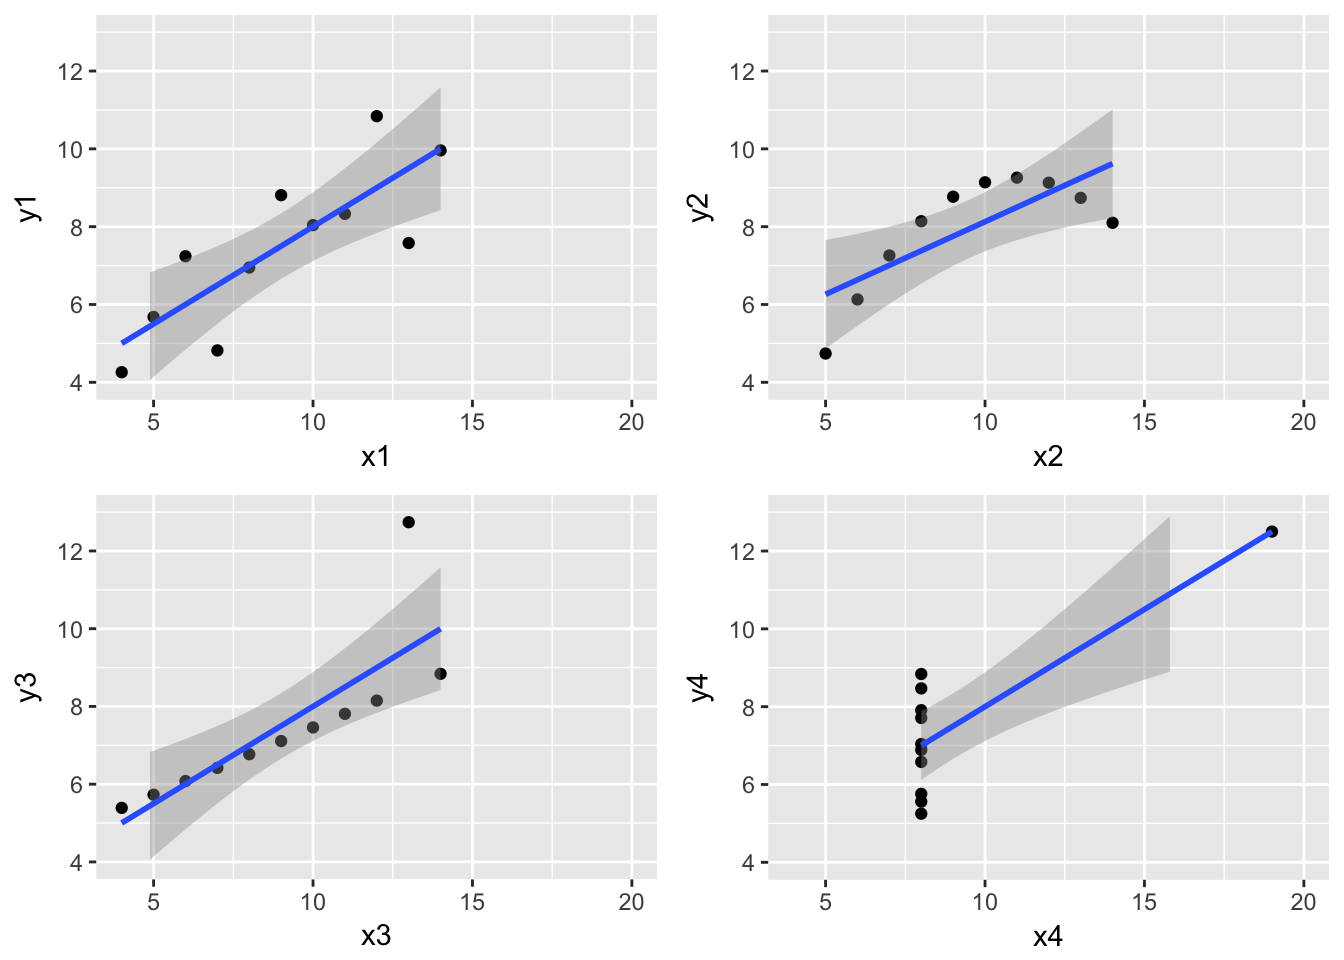
\includegraphics{eda_files/figure-latex/unnamed-chunk-7-1.pdf}

Interpretation of Scatter Plots Conclusions from the scatter plots are:

\begin{itemize}
\tightlist
\item
  data set 1 is clearly linear with some scatter.
\item
  data set 2 is clearly quadratic.
\item
  data set 3 clearly has an outlier.
\item
  data set 4 is obviously the victim of a poor experimental design with
  a single point far removed from the bulk of the data ``wagging the
  dog''.
\end{itemize}

Importance of Exploratory Analysis These points are exactly the
substance that provide and define ``insight'' and ``feel'' for a data
set. They are the goals and the fruits of an open exploratory data
analysis (EDA) approach to the data. Quantitative statistics are not
wrong per se, but they are incomplete. They are incomplete because they
are numeric summaries which in the summarization operation do a good job
of focusing on a particular aspect of the data (e.g., location,
intercept, slope, degree of relatedness, etc.) by judiciously reducing
the data to a few numbers. Doing so also filters the data, necessarily
omitting and screening out other sometimes crucial information in the
focusing operation. Quantitative statistics focus but also filter; and
filtering is exactly what makes the quantitative approach incomplete at
best and misleading at worst. The estimated intercepts (= 3) and slopes
(= 0.5) for data sets 2, 3, and 4 are misleading because the estimation
is done in the context of an assumed linear model and that linearity
assumption is the fatal flaw in this analysis.

The EDA approach of deliberately postponing the model selection until
further along in the analysis has many rewards, not the least of which
is the ultimate convergence to a much-improved model and the formulation
of valid and supportable scientific and engineering conclusions.

\subsection{General Problem
Categories}\label{general-problem-categories}

The following table is a convenient way to classify EDA problems.

\subsubsection{Univariate and Control}\label{univariate-and-control}

\begin{longtable}[]{@{}lll@{}}
\toprule
\begin{minipage}[b]{0.14\columnwidth}\raggedright\strut
Classification\strut
\end{minipage} & \begin{minipage}[b]{0.39\columnwidth}\raggedright\strut
Univariate\strut
\end{minipage} & \begin{minipage}[b]{0.39\columnwidth}\raggedright\strut
Control\strut
\end{minipage}\tabularnewline
\midrule
\endhead
\begin{minipage}[t]{0.14\columnwidth}\raggedright\strut
Data\strut
\end{minipage} & \begin{minipage}[t]{0.39\columnwidth}\raggedright\strut
A single column of numbers, Y.\strut
\end{minipage} & \begin{minipage}[t]{0.39\columnwidth}\raggedright\strut
A single column of numbers, Y.\strut
\end{minipage}\tabularnewline
\begin{minipage}[t]{0.14\columnwidth}\raggedright\strut
Model\strut
\end{minipage} & \begin{minipage}[t]{0.39\columnwidth}\raggedright\strut
y = constant + error\strut
\end{minipage} & \begin{minipage}[t]{0.39\columnwidth}\raggedright\strut
y = constant + error\strut
\end{minipage}\tabularnewline
\begin{minipage}[t]{0.14\columnwidth}\raggedright\strut
Output\strut
\end{minipage} & \begin{minipage}[t]{0.39\columnwidth}\raggedright\strut
- A number (the estimated constant in the model).- An estimate of
uncertainty for the constant.- An estimate of the distribution for the
error.\strut
\end{minipage} & \begin{minipage}[t]{0.39\columnwidth}\raggedright\strut
A ``yes'' or ``no'' to the question ``Is the system out of
control?''\strut
\end{minipage}\tabularnewline
\begin{minipage}[t]{0.14\columnwidth}\raggedright\strut
Techniques\strut
\end{minipage} & \begin{minipage}[t]{0.39\columnwidth}\raggedright\strut
4-PlotProbability PlotPPCC Plot\strut
\end{minipage} & \begin{minipage}[t]{0.39\columnwidth}\raggedright\strut
Control Charts\strut
\end{minipage}\tabularnewline
\bottomrule
\end{longtable}

\subsubsection{Comparative and
Screening}\label{comparative-and-screening}

\begin{longtable}[]{@{}lll@{}}
\toprule
\begin{minipage}[b]{0.14\columnwidth}\raggedright\strut
Classification\strut
\end{minipage} & \begin{minipage}[b]{0.39\columnwidth}\raggedright\strut
Comparative\strut
\end{minipage} & \begin{minipage}[b]{0.39\columnwidth}\raggedright\strut
Screening\strut
\end{minipage}\tabularnewline
\midrule
\endhead
\begin{minipage}[t]{0.14\columnwidth}\raggedright\strut
Data\strut
\end{minipage} & \begin{minipage}[t]{0.39\columnwidth}\raggedright\strut
A single response variable and k independent variables (Y,
X\textsubscript{1}, X\textsubscript{2}, \ldots{} , X\textsubscript{k}),
primary focus is on one (the primary factor) of these independent
variables.\strut
\end{minipage} & \begin{minipage}[t]{0.39\columnwidth}\raggedright\strut
A single response variable and k independent variables (Y,
X\textsubscript{1}, X\textsubscript{2}, \ldots{} ,
X\textsubscript{k}).\strut
\end{minipage}\tabularnewline
\begin{minipage}[t]{0.14\columnwidth}\raggedright\strut
Model\strut
\end{minipage} & \begin{minipage}[t]{0.39\columnwidth}\raggedright\strut
y = f(x\textsubscript{1}, x\textsubscript{2}, \ldots{},
x\textsubscript{k}) + error\strut
\end{minipage} & \begin{minipage}[t]{0.39\columnwidth}\raggedright\strut
y = f(x\textsubscript{1}, x\textsubscript{2}, \ldots{},
x\textsubscript{k}) + error\strut
\end{minipage}\tabularnewline
\begin{minipage}[t]{0.14\columnwidth}\raggedright\strut
Output\strut
\end{minipage} & \begin{minipage}[t]{0.39\columnwidth}\raggedright\strut
A ``yes'' or ``no'' to the question ``Is the primary factor
significant?''.\strut
\end{minipage} & \begin{minipage}[t]{0.39\columnwidth}\raggedright\strut
A ranked list (from most important to least important) of factors.Best
settings for the factors.A good model/prediction equation relating Y to
the factors.\strut
\end{minipage}\tabularnewline
\begin{minipage}[t]{0.14\columnwidth}\raggedright\strut
Techniques\strut
\end{minipage} & \begin{minipage}[t]{0.39\columnwidth}\raggedright\strut
Block PlotScatter PlotBox Plot\strut
\end{minipage} & \begin{minipage}[t]{0.39\columnwidth}\raggedright\strut
Block PlotProbability PlotBihistogram\strut
\end{minipage}\tabularnewline
\bottomrule
\end{longtable}

\subsubsection{Optimization and
Regression}\label{optimization-and-regression}

\begin{longtable}[]{@{}lll@{}}
\toprule
\begin{minipage}[b]{0.14\columnwidth}\raggedright\strut
Classification\strut
\end{minipage} & \begin{minipage}[b]{0.39\columnwidth}\raggedright\strut
Optimizatio\strut
\end{minipage} & \begin{minipage}[b]{0.39\columnwidth}\raggedright\strut
Regression\strut
\end{minipage}\tabularnewline
\midrule
\endhead
\begin{minipage}[t]{0.14\columnwidth}\raggedright\strut
Data\strut
\end{minipage} & \begin{minipage}[t]{0.39\columnwidth}\raggedright\strut
A single response variable and k independent variables (Y,
X\textsubscript{1}, X\textsubscript{2}, \ldots{} ,
X\textsubscript{k}).\strut
\end{minipage} & \begin{minipage}[t]{0.39\columnwidth}\raggedright\strut
A single response variable and k independent variables (Y,
X\textsubscript{1}, X\textsubscript{2}, \ldots{} ,
X\textsubscript{k})The independent variables can be continuous.\strut
\end{minipage}\tabularnewline
\begin{minipage}[t]{0.14\columnwidth}\raggedright\strut
Model\strut
\end{minipage} & \begin{minipage}[t]{0.39\columnwidth}\raggedright\strut
y = f(x\textsubscript{1}, x\textsubscript{2}, \ldots{},
x\textsubscript{k}) + error\strut
\end{minipage} & \begin{minipage}[t]{0.39\columnwidth}\raggedright\strut
y = f(x\textsubscript{1}, x\textsubscript{2}, \ldots{},
x\textsubscript{k}) + error\strut
\end{minipage}\tabularnewline
\begin{minipage}[t]{0.14\columnwidth}\raggedright\strut
Output\strut
\end{minipage} & \begin{minipage}[t]{0.39\columnwidth}\raggedright\strut
Best settings for the factor variables.\strut
\end{minipage} & \begin{minipage}[t]{0.39\columnwidth}\raggedright\strut
A good model/prediction equation relating Y to the factors.\strut
\end{minipage}\tabularnewline
\begin{minipage}[t]{0.14\columnwidth}\raggedright\strut
Techniques\strut
\end{minipage} & \begin{minipage}[t]{0.39\columnwidth}\raggedright\strut
Block PlotLeast Squares FittingContour Plot\strut
\end{minipage} & \begin{minipage}[t]{0.39\columnwidth}\raggedright\strut
Least Squares FittingScatter Plot6-Plot\strut
\end{minipage}\tabularnewline
\bottomrule
\end{longtable}

\subsubsection{Time Series and
Multivariate}\label{time-series-and-multivariate}

\begin{longtable}[]{@{}lll@{}}
\toprule
\begin{minipage}[b]{0.14\columnwidth}\raggedright\strut
Classification\strut
\end{minipage} & \begin{minipage}[b]{0.39\columnwidth}\raggedright\strut
Optimizatio\strut
\end{minipage} & \begin{minipage}[b]{0.39\columnwidth}\raggedright\strut
Regression\strut
\end{minipage}\tabularnewline
\midrule
\endhead
\begin{minipage}[t]{0.14\columnwidth}\raggedright\strut
Data\strut
\end{minipage} & \begin{minipage}[t]{0.39\columnwidth}\raggedright\strut
A column of time dependent numbers, Y. In addition, time is an
indpendent variable. The time variable can be either explicit or
implied. If the data are not equi-spaced, the time variable should be
explicitly provided.\strut
\end{minipage} & \begin{minipage}[t]{0.39\columnwidth}\raggedright\strut
k factor variables (X1, X2, \ldots{} , Xk).\strut
\end{minipage}\tabularnewline
\begin{minipage}[t]{0.14\columnwidth}\raggedright\strut
Model\strut
\end{minipage} & \begin{minipage}[t]{0.39\columnwidth}\raggedright\strut
y\textsubscript{t} = f(t) + errorThe model can be either a time domain
based or frequency domain based.\strut
\end{minipage} & \begin{minipage}[t]{0.39\columnwidth}\raggedright\strut
The model is not explicit.\strut
\end{minipage}\tabularnewline
\begin{minipage}[t]{0.14\columnwidth}\raggedright\strut
Output\strut
\end{minipage} & \begin{minipage}[t]{0.39\columnwidth}\raggedright\strut
A good model/prediction equation relating Y to previous values of
Y.\strut
\end{minipage} & \begin{minipage}[t]{0.39\columnwidth}\raggedright\strut
Identify underlying correlation structure in the data.\strut
\end{minipage}\tabularnewline
\begin{minipage}[t]{0.14\columnwidth}\raggedright\strut
Techniques\strut
\end{minipage} & \begin{minipage}[t]{0.39\columnwidth}\raggedright\strut
Autocorrelation PlotSpectrumComplex Demodulation Amplitude PlotComplex
Demodulation Phase PlotARIMA Models\strut
\end{minipage} & \begin{minipage}[t]{0.39\columnwidth}\raggedright\strut
Star PlotScatter Plot MatrixConditioning PlotProfile PlotPrincipal
ComponentsClusteringDiscrimination/Classification\strut
\end{minipage}\tabularnewline
\bottomrule
\end{longtable}

\section{EDA Assumptions}\label{eda-assumptions}

\subsection{Summary}\label{summary-1}

The gamut of scientific and engineering experimentation is virtually
limitless. In this sea of diversity is there any common basis that
allows the analyst to systematically and validly arrive at supportable,
repeatable research conclusions? Fortunately, there is such a basis and
it is rooted in the fact that every measurement process, however
complicated, has certain underlying assumptions. This section deals with
what those assumptions are, why they are important, how to go about
testing them, and what the consequences are if the assumptions do not
hold.

\subsection{Table of Contents for Section
2}\label{table-of-contents-for-section-2}

\begin{itemize}
\tightlist
\item
  Underlying Assumptions
\item
  Importance
\item
  Testing Assumptions
\item
  Importance of Plots
\item
  Consequences
\end{itemize}

\subsection{Underlying Assumptions}\label{underlying-assumptions}

\subsubsection{Assumptions Underlying a Measurement
Process}\label{assumptions-underlying-a-measurement-process}

There are four assumptions that typically underlie all measurement
processes; namely, that the data from the process at hand ``behave
like'':

\begin{itemize}
\tightlist
\item
  random drawings;
\item
  from a fixed distribution;
\item
  with the distribution having fixed location; and
\item
  with the distribution having fixed variation.
\end{itemize}

\subsubsection{Univariate or Single Response
Variable}\label{univariate-or-single-response-variable}

The ``fixed location'' referred to in item 3 above differs for different
problem types. The simplest problem type is univariate; that is, a
single variable. For the univariate problem, the general model
\textgreater{} response = deterministic component + random component
becomes \textgreater{} response = constant + error

\subsubsection{Assumptions for Univariate
Model}\label{assumptions-for-univariate-model}

For this case, the ``fixed location'' is simply the unknown constant. We
can thus imagine the process at hand to be operating under constant
conditions that produce a single column of data with the properties that

\begin{itemize}
\tightlist
\item
  the data are uncorrelated with one another;
\item
  the random component has a fixed distribution;
\item
  the deterministic component consists of only a constant; and
\item
  the random component has fixed variation.
\end{itemize}

\subsubsection{Extrapolation to a Function of Many
Variables}\label{extrapolation-to-a-function-of-many-variables}

The universal power and importance of the univariate model is that it
can easily be extended to the more general case where the deterministic
component is not just a constant, but is in fact a function of many
variables, and the engineering objective is to characterize and model
the function.

\subsubsection{Residuals Will Behave According to Univariate
Assumptions}\label{residuals-will-behave-according-to-univariate-assumptions}

The key point is that regardless of how many factors there are, and
regardless of how complicated the function is, if the engineer succeeds
in choosing a good model, then the differences (residuals) between the
raw response data and the predicted values from the fitted model should
themselves behave like a univariate process. Furthermore, the residuals
from this univariate process fit will behave like: random drawings; from
a fixed distribution; with fixed location (namely, 0 in this case); and
with fixed variation. Validation of Model Thus if the residuals from the
fitted model do in fact behave like the ideal, then testing of
underlying assumptions becomes a tool for the validation and quality of
fit of the chosen model. On the other hand, if the residuals from the
chosen fitted model violate one or more of the above univariate
assumptions, then the chosen fitted model is inadequate and an
opportunity exists for arriving at an improved model.

\subsection{Importance}\label{importance}

\subsubsection{Predictability and Statistical
Control}\label{predictability-and-statistical-control}

Predictability is an all-important goal in science and engineering. If
the four underlying assumptions hold, then we have achieved
probabilistic predictability--the ability to make probability statements
not only about the process in the past, but also about the process in
the future. In short, such processes are said to be ``in statistical
control''.

\subsubsection{Validity of Engineering}\label{validity-of-engineering}

Conclusions Moreover, if the four assumptions are valid, then the
process is amenable to the generation of valid scientific and
engineering conclusions. If the four assumptions are not valid, then the
process is drifting (with respect to location, variation, or
distribution), unpredictable, and out of control. A simple
characterization of such processes by a location estimate, a variation
estimate, or a distribution ``estimate'' inevitably leads to engineering
conclusions that are not valid, are not supportable (scientifically or
legally), and which are not repeatable in the laboratory.

\subsection{Techniques for Testing
Assumptions}\label{techniques-for-testing-assumptions}

\subsubsection{Testing Underlying Assumptions Helps Assure the Validity
of Scientific and Engineering
Conclusions}\label{testing-underlying-assumptions-helps-assure-the-validity-of-scientific-and-engineering-conclusions}

Because the validity of the final scientific/engineering conclusions is
inextricably linked to the validity of the underlying univariate
assumptions, it naturally follows that there is a real necessity that
each and every one of the above four assumptions be routinely tested.

Four Techniques to Test Underlying Assumptions\\
The following EDA techniques are simple, efficient, and powerful for the
routine testing of underlying assumptions:

\begin{enumerate}
\def\labelenumi{\arabic{enumi}.}
\tightlist
\item
  run sequence plot (Yi versus i)
\item
  lag plot (Yi versus Yi-1)
\item
  histogram (counts versus subgroups of Y)
\item
  normal probability plot (ordered Y versus theoretical ordered Y)
\end{enumerate}

\subsubsection{Plot on a Single Page for a Quick Characterization of the
Data}\label{plot-on-a-single-page-for-a-quick-characterization-of-the-data}

The four EDA plots can be juxtaposed for a quick look at the
characteristics of the data. The plots below are ordered as follows:

\begin{itemize}
\tightlist
\item
  Run sequence plot - upper left
\item
  Lag plot - upper right
\item
  Histogram - lower left
\item
  Normal probability plot - lower right
\end{itemize}

\subsubsection{Sample Plot: Assumptions
Hold}\label{sample-plot-assumptions-hold}

A 4-Plot which shows fixed location, fixed variation, fixed normal
distribution, and no outliers

\begin{Shaded}
\begin{Highlighting}[]
\CommentTok{#insert 4-plot}
\KeywordTok{library}\NormalTok{(tidyverse)}
\NormalTok{four_plot <-}\StringTok{ }\ControlFlowTok{function}\NormalTok{ (y)\{}
  \CommentTok{# take in a numeric verctor for univariate analysis}
  \ControlFlowTok{if}\NormalTok{(}\OperatorTok{!}\StringTok{ }\KeywordTok{is.numeric}\NormalTok{(y)) }\KeywordTok{stop}\NormalTok{(}\StringTok{"Requires a numeric vector"}\NormalTok{)}
\NormalTok{  da <-}\StringTok{ }\KeywordTok{tibble}\NormalTok{( }\DataTypeTok{idx =} \DecValTok{1}\OperatorTok{:}\KeywordTok{length}\NormalTok{(y), y )}
\NormalTok{  p1 =}\StringTok{ }\KeywordTok{ggplot}\NormalTok{(da, }\KeywordTok{aes}\NormalTok{(}\DataTypeTok{x=}\NormalTok{idx, }\DataTypeTok{y=}\NormalTok{y)) }\OperatorTok{+}\StringTok{ }\KeywordTok{geom_line}\NormalTok{() }\CommentTok{# run sequenc}
\NormalTok{  p2 =}\StringTok{ }\KeywordTok{ggplot}\NormalTok{(da, }\KeywordTok{aes}\NormalTok{(}\DataTypeTok{x =}\NormalTok{ y, }\DataTypeTok{y =} \KeywordTok{c}\NormalTok{(}\KeywordTok{tail}\NormalTok{(y, }\OperatorTok{-}\DecValTok{1}\NormalTok{),}\DecValTok{0}\NormalTok{))) }\OperatorTok{+}\StringTok{ }\KeywordTok{geom_point}\NormalTok{() }\CommentTok{# lag plot}
\NormalTok{  p3 =}\StringTok{ }\KeywordTok{ggplot}\NormalTok{(da, }\KeywordTok{aes}\NormalTok{(}\DataTypeTok{x=}\NormalTok{y)) }\OperatorTok{+}\StringTok{ }\KeywordTok{geom_histogram}\NormalTok{() }\CommentTok{#histogram}
\NormalTok{  p4 <-}\StringTok{ }\KeywordTok{ggplot}\NormalTok{(da, }\KeywordTok{aes}\NormalTok{(}\DataTypeTok{sample=}\NormalTok{y)) }\OperatorTok{+}\StringTok{ }\KeywordTok{geom_qq}\NormalTok{() }\CommentTok{# qqplot}
\NormalTok{  gridExtra}\OperatorTok{::}\KeywordTok{grid.arrange}\NormalTok{(p1, p2, p3, p4, }\DataTypeTok{ncol =} \DecValTok{2}\NormalTok{)}
\NormalTok{\}}

\KeywordTok{four_plot}\NormalTok{(}\KeywordTok{rnorm}\NormalTok{(}\DecValTok{500}\NormalTok{))}
\end{Highlighting}
\end{Shaded}

\begin{verbatim}
## `stat_bin()` using `bins = 30`. Pick better value with `binwidth`.
\end{verbatim}

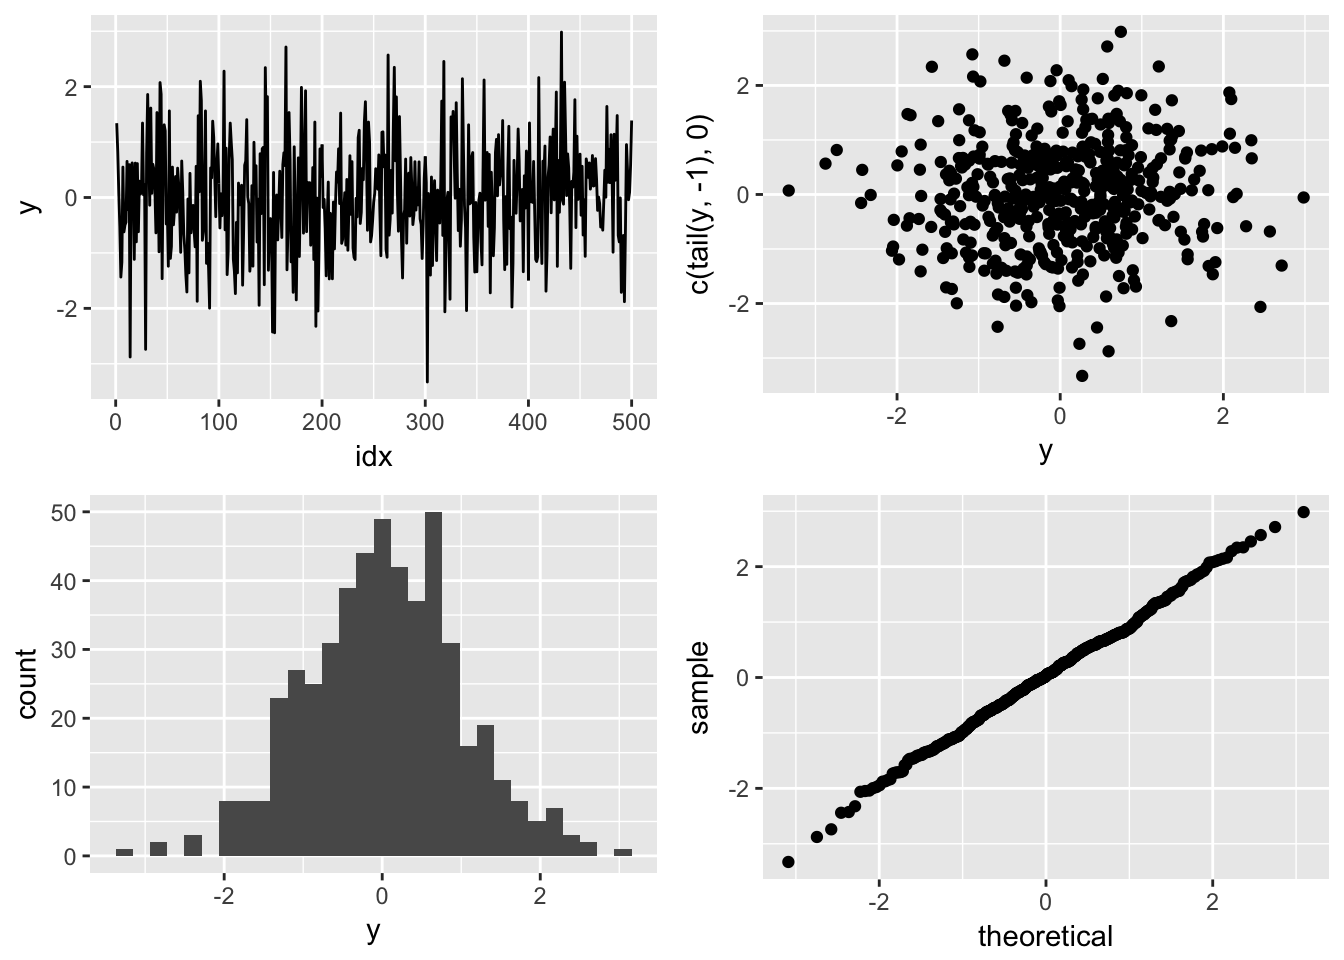
\includegraphics{eda_files/figure-latex/unnamed-chunk-8-1.pdf} This
4-plot of 500 normal random numbers reveals a process that has fixed
location, fixed variation, is random, apparently has a fixed
approximately normal distribution, and has no outliers.

\subsubsection{Sample Plot: Assumptions Do Not
Hold}\label{sample-plot-assumptions-do-not-hold}

If one or more of the four underlying assumptions do not hold, then it
will show up in the various plots as demonstrated in the following
example.

\begin{Shaded}
\begin{Highlighting}[]
\NormalTok{LEW <-}\StringTok{ }\KeywordTok{read_csv}\NormalTok{(}\StringTok{"~/Dropbox/github/R_Codes_and_Data/Rdata/LEW.DAT"}\NormalTok{, }
     \DataTypeTok{col_names =} \OtherTok{FALSE}\NormalTok{, }\DataTypeTok{col_types =} \KeywordTok{cols}\NormalTok{(}\DataTypeTok{X1 =} \KeywordTok{col_double}\NormalTok{()), }\DataTypeTok{skip =} \DecValTok{25}\NormalTok{)}
\KeywordTok{names}\NormalTok{(LEW) <-}\StringTok{ }\KeywordTok{c}\NormalTok{(}\StringTok{"deflection"}\NormalTok{)}
\KeywordTok{four_plot}\NormalTok{(LEW}\OperatorTok{$}\NormalTok{deflection)}
\end{Highlighting}
\end{Shaded}

\begin{verbatim}
## `stat_bin()` using `bins = 30`. Pick better value with `binwidth`.
\end{verbatim}

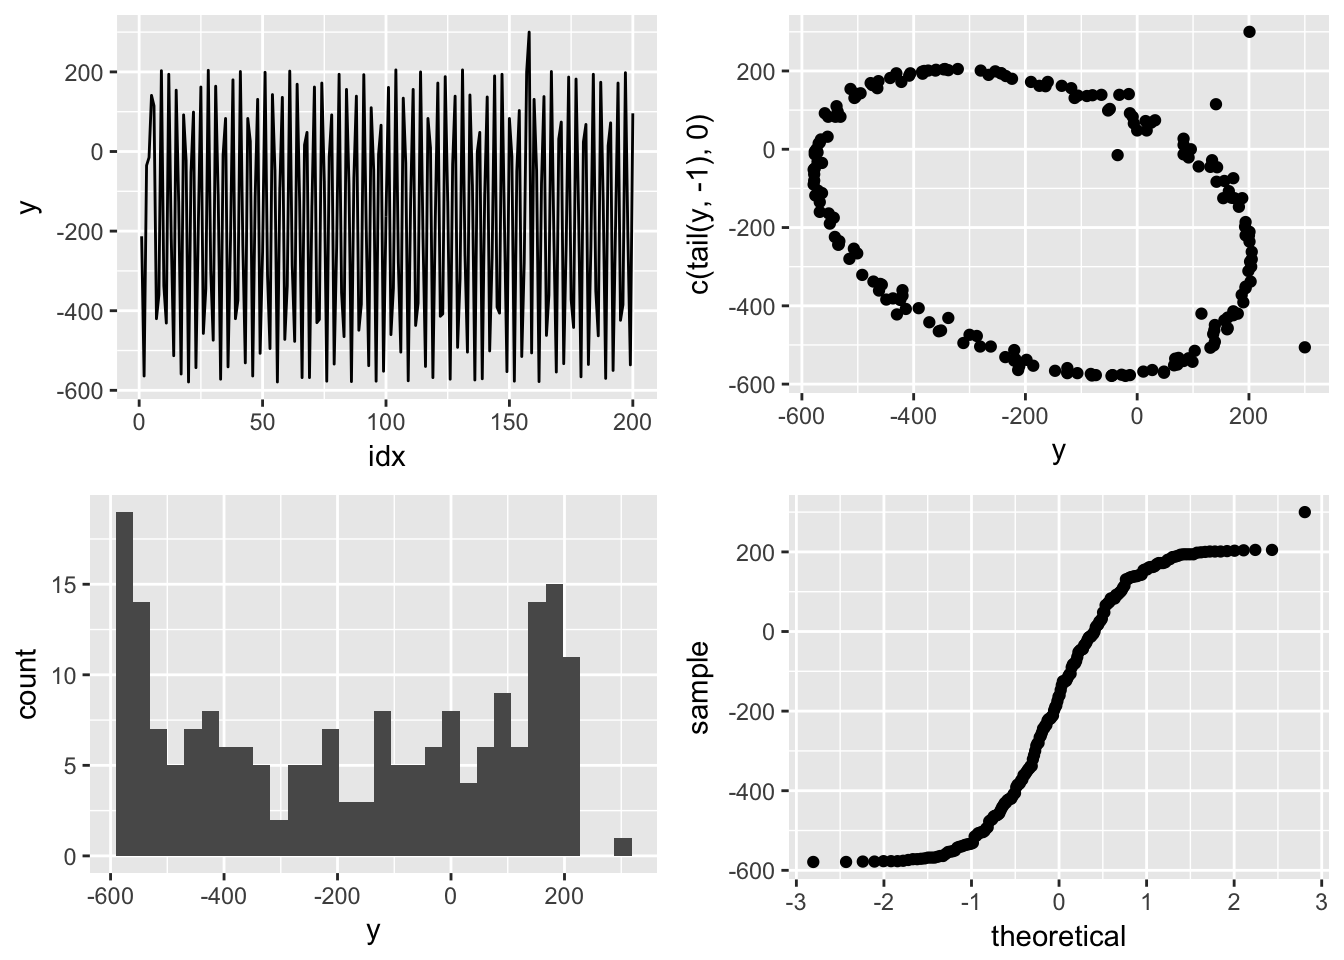
\includegraphics{eda_files/figure-latex/unnamed-chunk-9-1.pdf}

This 4-plot reveals a process that has fixed location, fixed variation,
is non-random (oscillatory), has a non-normal, U-shaped distribution,
and has several outliers.

\subsection{Interpretation of 4-Plot}\label{interpretation-of-4-plot}

\subsubsection{Interpretation of EDA Plots: Flat and Equi-Banded,
Random, Bell-Shaped, and
Linear}\label{interpretation-of-eda-plots-flat-and-equi-banded-random-bell-shaped-and-linear}

The four EDA plots discussed on the previous page are used to test the
underlying assumptions:

\textbf{- Fixed Location:} If the fixed location assumption holds, then
the run sequence plot will be flat and non-drifting.

\textbf{- Fixed Variation:} If the fixed variation assumption holds,
then the vertical spread in the run sequence plot will be the
approximately the same over the entire horizontal axis.

\textbf{- Randomness:} If the randomness assumption holds, then the lag
plot will be structureless and random.

\textbf{- Fixed Distribution:} If the fixed distribution assumption
holds, in particular if the fixed normal distribution holds, then

\begin{enumerate}
\def\labelenumi{\arabic{enumi}.}
\tightlist
\item
  the histogram will be bell-shaped, and
\item
  the normal probability plot will be linear.
\end{enumerate}

\subsubsection{Plots Utilized to Test the
Assumptions}\label{plots-utilized-to-test-the-assumptions}

Conversely, the underlying assumptions are tested using the EDA plots:

\textbf{- Run Sequence Plot:} If the run sequence plot is flat and
non-drifting, the fixed-location assumption holds. If the run sequence
plot has a vertical spread that is about the same over the entire plot,
then the fixed-variation assumption holds.

\textbf{- Lag Plot:} If the lag plot is structureless, then the
randomness assumption holds.

\textbf{- Histogram:} If the histogram is bell-shaped, the underlying
distribution is symmetric and perhaps approximately normal.

\textbf{- Normal Probability Plot:} If the normal probability plot is
linear, the underlying distribution is approximately normal.

If all four of the assumptions hold, then the process is said
definitionally to be ``in statistical control''.

\begin{center}\rule{0.5\linewidth}{\linethickness}\end{center}

You can label chapter and section titles using \texttt{\{\#label\}}
after them, e.g., we can reference Chapter \ref{intro}. If you do not
manually label them, there will be automatic labels anyway, e.g.,
Chapter \ref{methods}.

Figures and tables with captions will be placed in \texttt{figure} and
\texttt{table} environments, respectively.

\begin{Shaded}
\begin{Highlighting}[]
\KeywordTok{par}\NormalTok{(}\DataTypeTok{mar =} \KeywordTok{c}\NormalTok{(}\DecValTok{4}\NormalTok{, }\DecValTok{4}\NormalTok{, .}\DecValTok{1}\NormalTok{, .}\DecValTok{1}\NormalTok{))}
\KeywordTok{plot}\NormalTok{(pressure, }\DataTypeTok{type =} \StringTok{'b'}\NormalTok{, }\DataTypeTok{pch =} \DecValTok{19}\NormalTok{)}
\end{Highlighting}
\end{Shaded}

\begin{figure}

{\centering 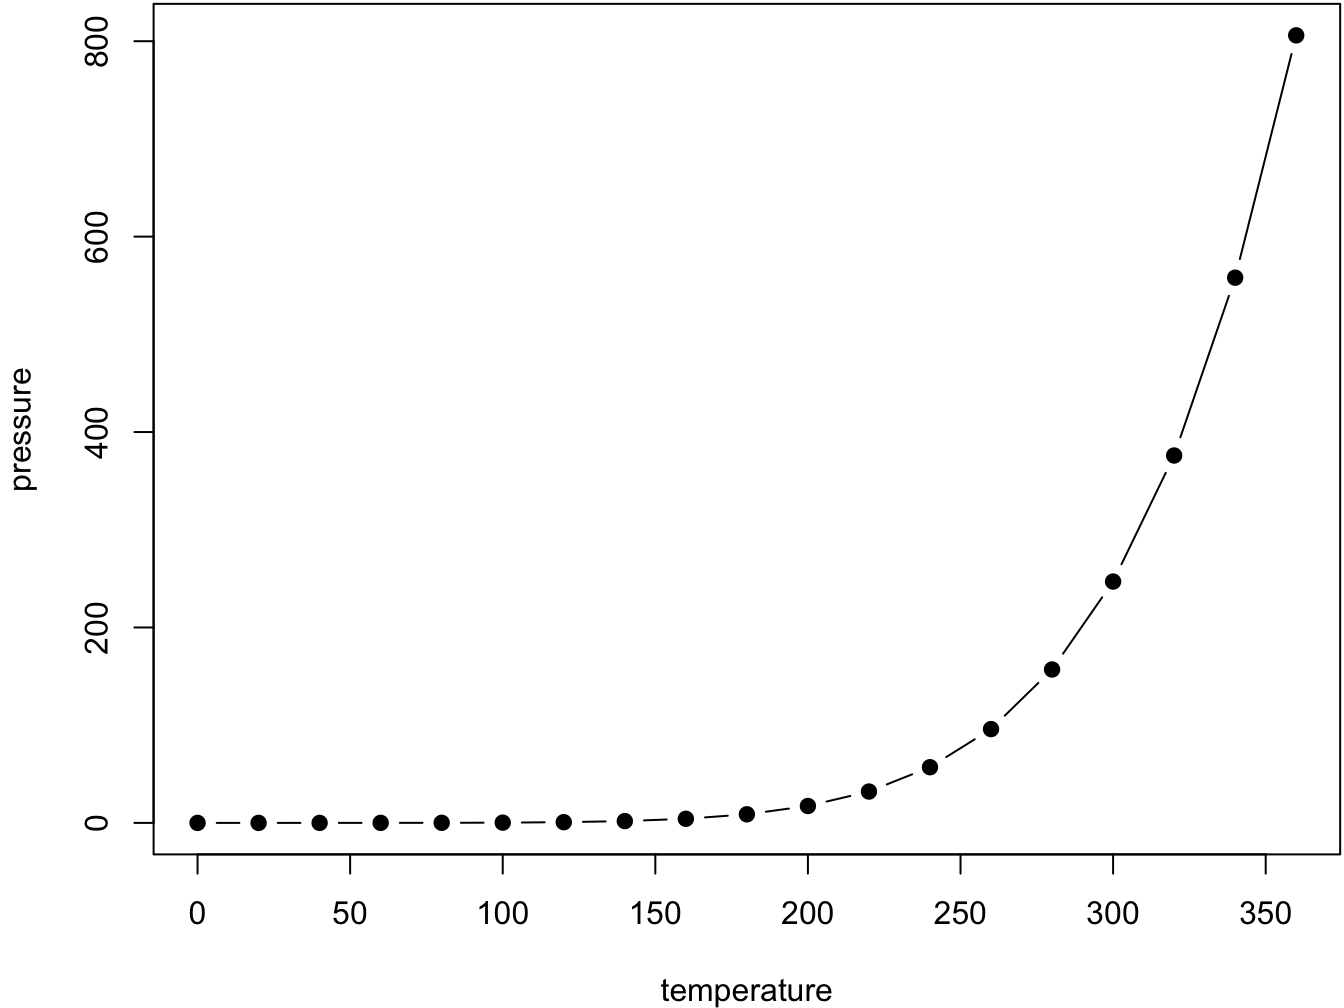
\includegraphics[width=0.8\linewidth]{eda_files/figure-latex/nice-fig-1} 

}

\caption{Here is a nice figure!}\label{fig:nice-fig}
\end{figure}

Reference a figure by its code chunk label with the \texttt{fig:}
prefix, e.g., see Figure \ref{fig:nice-fig}. Similarly, you can
reference tables generated from \texttt{knitr::kable()}, e.g., see Table
\ref{tab:nice-tab}.

\begin{Shaded}
\begin{Highlighting}[]
\NormalTok{knitr}\OperatorTok{::}\KeywordTok{kable}\NormalTok{(}
  \KeywordTok{head}\NormalTok{(iris, }\DecValTok{20}\NormalTok{), }\DataTypeTok{caption =} \StringTok{'Here is a nice table!'}\NormalTok{,}
  \DataTypeTok{booktabs =} \OtherTok{TRUE}
\NormalTok{)}
\end{Highlighting}
\end{Shaded}

\begin{table}

\caption{\label{tab:nice-tab}Here is a nice table!}
\centering
\begin{tabular}[t]{rrrrl}
\toprule
Sepal.Length & Sepal.Width & Petal.Length & Petal.Width & Species\\
\midrule
5.1 & 3.5 & 1.4 & 0.2 & setosa\\
4.9 & 3.0 & 1.4 & 0.2 & setosa\\
4.7 & 3.2 & 1.3 & 0.2 & setosa\\
4.6 & 3.1 & 1.5 & 0.2 & setosa\\
5.0 & 3.6 & 1.4 & 0.2 & setosa\\
\addlinespace
5.4 & 3.9 & 1.7 & 0.4 & setosa\\
4.6 & 3.4 & 1.4 & 0.3 & setosa\\
5.0 & 3.4 & 1.5 & 0.2 & setosa\\
4.4 & 2.9 & 1.4 & 0.2 & setosa\\
4.9 & 3.1 & 1.5 & 0.1 & setosa\\
\addlinespace
5.4 & 3.7 & 1.5 & 0.2 & setosa\\
4.8 & 3.4 & 1.6 & 0.2 & setosa\\
4.8 & 3.0 & 1.4 & 0.1 & setosa\\
4.3 & 3.0 & 1.1 & 0.1 & setosa\\
5.8 & 4.0 & 1.2 & 0.2 & setosa\\
\addlinespace
5.7 & 4.4 & 1.5 & 0.4 & setosa\\
5.4 & 3.9 & 1.3 & 0.4 & setosa\\
5.1 & 3.5 & 1.4 & 0.3 & setosa\\
5.7 & 3.8 & 1.7 & 0.3 & setosa\\
5.1 & 3.8 & 1.5 & 0.3 & setosa\\
\bottomrule
\end{tabular}
\end{table}

You can write citations, too. For example, we are using the
\textbf{bookdown} package \citep{R-bookdown} in this sample book, which
was built on top of R Markdown and \textbf{knitr} \citep{xie2015}.

\chapter{Measurement Process
Characterization}\label{measurement-process-characterization}

\section{Characterization}\label{characterization}

The primary goal of this section is to lay the groundwork for
understanding the measurement process in terms of the errors that affect
the process.

What are the issues for characterization?

\begin{itemize}
\tightlist
\item
  Purpose
\item
  Reference base
\item
  Bias and Accuracy
\item
  Variability
\item
  What is a check standard?
\end{itemize}

Assumptions - Data collection - Analysis

\chapter{Methods}\label{methods}

We describe our methods in this chapter.

\chapter{Applications}\label{applications}

Some \emph{significant} applications are demonstrated in this chapter.

\section{Example one}\label{example-one}

\section{Example two}\label{example-two}

\chapter{Final Words}\label{final-words}

We have finished a nice book.

\section{Introduction}\label{introduction}

This section introduces the terminology and models that will be used to
describe and quantify product reliability. The terminology, probability
distributions and models used for reliability analysis differ in many
cases from those used in other statistical applications.

\subsection{Why is the assessment and control of product reliability
important?}\label{why-is-the-assessment-and-control-of-product-reliability-important}

\begin{quote}
We depend on, demand, and expect reliable products
\end{quote}

In today's technological world nearly everyone depends upon the
continued functioning of a wide array of complex machinery and equipment
for their everyday health, safety, mobility and economic welfare. We
expect our cars, computers, electrical appliances, lights, televisions,
etc. to function whenever we need them - day after day, year after year.
When they fail the results can be catastrophic: injury, loss of life
and/or costly lawsuits can occur. More often, repeated failure leads to
annoyance, inconvenience and a lasting customer dissatisfaction that can
play havoc with the responsible company's marketplace position.

\begin{quote}
Shipping unreliable products can destroy a company's reputation
\end{quote}

It takes a long time for a company to build up a reputation for
reliability, and only a short time to be branded as ``unreliable'' after
shipping a flawed product. Continual assessment of new product
reliability and ongoing control of the reliability of everything shipped
are critical necessities in today's competitive business arena.

\subsubsection{Quality versus
reliability}\label{quality-versus-reliability}

\begin{quote}
Reliability is ``quality changing over time''
\end{quote}

The everyday usage term ``quality of a product'' is loosely taken to
mean its inherent degree of excellence. In industry, this is made more
precise by defining quality to be ``conformance to requirements at the
start of use''. Assuming the product specifications adequately capture
customer requirements, the quality level can now be precisely measured
by the fraction of units shipped that meet specifications.

\begin{quote}
A motion picture instead of a snapshot
\end{quote}

But how many of these units still meet specifications after a week of
operation? Or after a month, or at the end of a one year warranty
period? That is where ``reliability'' comes in. Quality is a snapshot at
the start of life and reliability is a motion picture of the day-by-day
operation. Time zero defects are manufacturing mistakes that escaped
final test. The additional defects that appear over time are
``reliability defects'' or reliability fallout.

\begin{quote}
Life distributions model fraction fallout over time
\end{quote}

The quality level might be described by a single fraction defective. To
describe reliability fallout a probability model that describes the
fraction fallout over time is needed. This is known as the life
distribution model.

\subsubsection{Competitive driving
factors}\label{competitive-driving-factors}

\begin{quote}
Reliability is a major economic factor in determining a product's
success
\end{quote}

Accurate prediction and control of reliability plays an important role
in the profitability of a product. Service costs for products within the
warranty period or under a service contract are a major expense and a
significant pricing factor. Proper spare part stocking and support
personnel hiring and training also depend upon good reliability fallout
predictions. On the other hand, missing reliability targets may invoke
contractual penalties and cost future business. Companies that can
economically design and market products that meet their customers'
reliability expectations have a strong competitive advantage in today's
marketplace.

\subsubsection{Safety and health
considerations}\label{safety-and-health-considerations}

\begin{quote}
Some failures have serious social consequences and this should be taken
into account when planning reliability studies
\end{quote}

Sometimes equipment failure can have a major impact on human safety
and/or health. Automobiles, planes, life support equipment, and power
generating plants are a few examples. From the point of view of
``assessing product reliability'', we treat these kinds of catastrophic
failures no differently from the failure that occurs when a key
parameter measured on a manufacturing tool drifts slightly out of
specification, calling for an unscheduled maintenance action.

It is up to the reliability engineer (and the relevant customer) to
define what constitutes a failure in any reliability study. More
resource (test time and test units) should be planned for when an
incorrect reliability assessment could negatively impact safety and/or
health.

\subsection{What are the basic terms and models used for reliability
evaluation?}\label{what-are-the-basic-terms-and-models-used-for-reliability-evaluation}

\begin{quote}
Reliability methods and terminology began with 19th century insurance
companies
\end{quote}

Reliability theory developed apart from the mainstream of probability
and statistics, and was used primarily as a tool to help nineteenth
century maritime and life insurance companies compute profitable rates
to charge their customers. Even today, the terms ``failure rate'' and
``hazard rate'' are often used interchangeably. The following sections
will define some of the concepts, terms, and models we need to describe,
estimate and predict reliability.

\subsubsection{Repairable systems, non-repairable populations and
lifetime distribution
models}\label{repairable-systems-non-repairable-populations-and-lifetime-distribution-models}

\begin{quote}
Life distribution models describe how non-repairable populations fail
over time
\end{quote}

A repairable system is one which can be restored to satisfactory
operation by any action, including parts replacements or changes to
adjustable settings. When discussing the rate at which failures occur
during system operation time (and are then repaired) we will define a
Rate of Occurrence of Failure (ROCF) or ``repair rate''. It would be
incorrect to talk about failure rates or hazard rates for repairable
systems, as these terms apply only to the first failure times for a
population of non repairable components. A non-repairable population is
one for which individual items that fail are removed permanently from
the population. While the system may be repaired by replacing failed
units from either a similar or a different population, the members of
the original population dwindle over time until all have eventually
failed.

We begin with models and definitions for non-repairable populations.
Repair rates for repairable populations will be defined in a later
section.

The theoretical population models used to describe unit lifetimes are
known as \textbf{Lifetime Distribution Models}. The population is
generally considered to be all of the possible unit lifetimes for all of
the units that could be manufactured based on a particular design and
choice of materials and manufacturing process. A random sample of size
\emph{n} from this population is the collection of failure times
observed for a randomly selected group of \emph{n} units.

\begin{quote}
Any continuous PDF defined only for non-negative values can be a
lifetime distribution model
\end{quote}

A lifetime distribution model can be any probability density function
(or PDF) f(t) defined over the range of time from t=0,\ldots{},∞. The
corresponding cumulative distribution function (or CDF) F(t) is a very
useful function, as it gives the probability that a randomly selected
unit will fail by time t. The figure below shows the relationship
between f(t) and F(t) and gives three descriptions of F(t).

\begin{figure}
\centering
\includegraphics{http://www.itl.nist.gov/div898/handbook/apr/section1/gifs/f81212.gif}
\caption{PDF}
\end{figure}

\begin{enumerate}
\def\labelenumi{\arabic{enumi}.}
\tightlist
\item
  F(t) = the area under the PDF f(t) to the left of t.
\item
  F(t) = the probability that a single randomly chosen new unit will
  fail by time t.
\item
  F(t) = the proportion of the entire population that fails by time t.
\end{enumerate}

The figure above also shows a shaded area under \(f(t)\) between the two
times \(t_1\) and \(t_2\). This area is \([F(t2)−F(t1)]\) and represents
the proportion of the population that fails between times \(t_1\) and
\(t_2\) (or the probability that a brand new randomly chosen unit will
survive to time \(t_1\) but fail before time \(t_2\)). Note that the PDF
\(f(t)\) has only non-negative values and eventually either becomes 0 as
t increases, or decreases towards 0. The CDF \(F(t)\) is monotonically
increasing and goes from 0 to 1 as t approaches infinity. In other
words, the total area under the curve is always 1.

\begin{quote}
The Weibull model is a good example of a life distribution
\end{quote}

The 2-parameter Weibull distribution is an example of a popular
\(F(t)\). It has the CDF and PDF equations given by:
\[F(t)= 1-e^{-(t/\alpha)^\gamma}\]
\[f(t)=\frac{\gamma}{t} \left(\frac{t}{\alpha} \right)^\gamma e^{-(t/\alpha)^\gamma}\]
where \(\gamma\) is the ``shape'' parameter and \(\alpha\) is a
``scale'' parameter called the characteristic life. Example: A company
produces automotive fuel pumps that fail according to a Weibull life
distribution model with shape parameter \(\gamma=1.5\) and scale
parameter 8,000 (time measured in use hours). If a typical pump is used
800 hours a year, what proportion are likely to fail within 5 years?

Solution: The probability associated with the 800*5 quantile of a
Weibull distribution with \(\gamma=1.5\) and \(\alpha=8000\) is
0.2978115. Thus about 30\% of the pumps will fail in the first 5 years.

Functions for computing PDF values and CDF values, are available in both
Dataplot code and R code.

\begin{Shaded}
\begin{Highlighting}[]
\KeywordTok{print}\NormalTok{((}\KeywordTok{paste}\NormalTok{(}\StringTok{"The probability associated with the 800*5 quantile of a Weibull distribution with gamma=1.5 and alpha=8000 is"}\NormalTok{, }\KeywordTok{as.character}\NormalTok{(}\KeywordTok{pweibull}\NormalTok{(}\DecValTok{800}\OperatorTok{*}\DecValTok{5}\NormalTok{, }\FloatTok{1.5}\NormalTok{, }\DecValTok{8000}\NormalTok{)))))}
\end{Highlighting}
\end{Shaded}

\begin{verbatim}
## [1] "The probability associated with the 800*5 quantile of a Weibull distribution with gamma=1.5 and alpha=8000 is 0.29781149867344"
\end{verbatim}

\begin{Shaded}
\begin{Highlighting}[]
\KeywordTok{print}\NormalTok{(}\KeywordTok{paste}\NormalTok{(}\StringTok{"Thus about"}\NormalTok{, }\KeywordTok{paste0}\NormalTok{(}\KeywordTok{as.character}\NormalTok{(}\KeywordTok{round}\NormalTok{(}\KeywordTok{pweibull}\NormalTok{(}\DecValTok{800}\OperatorTok{*}\DecValTok{5}\NormalTok{, }\FloatTok{1.5}\NormalTok{, }\DecValTok{8000}\NormalTok{)}\OperatorTok{*}\DecValTok{100}\NormalTok{, }\DataTypeTok{digits =} \DecValTok{0}\NormalTok{)), }\StringTok{"%"}\NormalTok{),  }\StringTok{"of the pumps will fail in the first 5 years."}\NormalTok{))}
\end{Highlighting}
\end{Shaded}

\begin{verbatim}
## [1] "Thus about 30% of the pumps will fail in the first 5 years."
\end{verbatim}

\subsubsection{Reliability or survival
function}\label{reliability-or-survival-function}

\begin{quote}
Survival is the complementary event to failure
\end{quote}

The Reliability Function \(R(t)\), also known as the Survival Function
\(S(t)\), is defined by R(t)=S(t)=the probability a unit survives beyond
time t. Since a unit either fails, or survives, and one of these two
mutually exclusive alternatives must occur, we have \[R(t)=1−F(t)\]
\[F(t)=1−R(t)\].

\begin{quote}
The reliability of the system is the product of the reliability
functions of the components
\end{quote}

Calculations using R(t) often occur when building up from single
components to subsystems with many components. For example, if one
microprocessor comes from a population with reliability function
\(R_{m}(t)\) and two of them are used for the CPU in a system, then the
system CPU has a reliability function given by \[R_{cpu}(t) = R_m^2(t)\]
since both must survive in order for the system to survive. This
building up to the system from the individual components will be
discussed in detail when we look at the ``Bottom-Up'' method. The
general rule is: to calculate the reliability of a system of independent
components, multiply the reliability functions of all the components
together.

\subsubsection{Failure (or hazard) rate}\label{failure-or-hazard-rate}

\begin{quote}
The failure rate is the rate at which the population survivors at any
given instant are ``falling over the cliff''
\end{quote}

The failure rate is defined for non repairable populations as the
(instantaneous) rate of failure for the survivors to time t during the
next instant of time. It is a rate per unit of time similar in meaning
to reading a car speedometer at a particular instant and seeing 45 mph.
The next instant the failure rate may change and the units that have
already failed play no further role since only the survivors count. The
failure rate (or hazard rate) is denoted by h(t) and is calculated from
\[h(t) = \frac{f(t)}{1 - F(t)} = \frac{f(t)}{R(t)} = \mbox{the instantaneous (conditional) failure rate.}\]
The failure rate is sometimes called a ``conditional failure rate''
since the denominator \(1−F(t)\) (i.e., the population survivors)
converts the expression into a conditional rate, given survival past
time t. Since \(h(t)\) is also equal to the negative of the derivative
of \(ln[R(t)]\), we have the useful identity:
\[F(t)=1-\mbox{exp}\left[-\int_0^t h(t)dt\right]\] If we let
\[H(t) = \int_0^t h(t)dt\]

be the Cumulative Hazard Function, we then have \(F(t)=1−e^{H(t)}\). Two
other useful identities that follow from these formulas are:
\[h(t) = - \frac{d \mbox{ln} R(t)}{dt}\] \[H(t) = - \mbox{ln} R(t)\]

It is also sometimes useful to define an average failure rate over any
interval (T\textsubscript{1},T\textsubscript{2}) that ``averages'' the
failure rate over that interval. This rate, denoted by
AFR(T\textsubscript{1},T\textsubscript{2}), is a single number that can
be used as a specification or target for the population failure rate
over that interval. If T\textsubscript{1} is 0, it is dropped from the
expression. Thus, for example, AFR(40,000) would be the average failure
rate for the population over the first 40,000 hours of operation.

The formulas for calculating \emph{AFR} values are:
\[AFR(T_2 - T_1) = \frac{\int_{T_1}^{T_2} h(t)dt}{T_2 - T_1} = \frac{H(T_2) - H(T_1)}{T_2 - T_1} = \frac{\mbox{ln}R(T_1) - \mbox{ln}R(T_2)}{T_2 - T_1}\]

and \[AFR(0,T) = AFR(T) = \frac{H(T)}{T} = \frac{-\mbox{ln} R(T)}{T}\]

\subsubsection{\texorpdfstring{``Bathtub''
curve}{Bathtub curve}}\label{bathtub-curve}

\begin{quote}
A plot of the failure rate over time for most products yields a curve
that looks like a drawing of a bathtub
\end{quote}

If enough units from a given population are observed operating and
failing over time, it is relatively easy to compute week-by-week (or
month-by-month) estimates of the failure rate \(h(t)\). For example, if
\(N_{12}\) units survive to start the 13th month of life and \(r_{13}\)
of them fail during the next month (or 720 hours) of life, then a simple
empirical estimate of \(h(t)\) averaged across the 13th month of life
(or between 8640 hours and 9360 hours of age), is given by
\((\frac{r_{13}} {N_{12}}⋅720)\). Similar estimates are discussed in
detail in the section on Empirical Model Fitting.

Over many years, and across a wide variety of mechanical and electronic
components and systems, people have calculated empirical population
failure rates as units age over time and repeatedly obtained a graph
such as shown below. Because of the shape of this failure rate curve, it
has become widely known as the ``Bathtub'' curve.

The initial region that begins at time zero when a customer first begins
to use the product is characterized by a high but rapidly decreasing
failure rate. This region is known as the \textbf{Early Failure Period}
(also referred to as \textbf{Infant Mortality Period}, from the
actuarial origins of the first bathtub curve plots). This decreasing
failure rate typically lasts several weeks to a few months.

Next, the failure rate levels off and remains roughly constant for
(hopefully) the majority of the useful life of the product. This long
period of a level failure rate is known as the \textbf{Intrinsic Failure
Period} (also called the \textbf{Stable Failure Period}) and the
constant failure rate level is called the \textbf{Intrinsic Failure
Rate}. Note that most systems spend most of their lifetimes operating in
this flat portion of the bathtub curve

Finally, if units from the population remain in use long enough, the
failure rate begins to increase as materials wear out and degradation
failures occur at an ever increasing rate. This is the \textbf{Wearout
Failure Period}.

\begin{figure}
\centering
\includegraphics{http://www.itl.nist.gov/div898/handbook/apr/section1/gifs/bathtub2.gif}
\caption{Bathtub Curve}
\end{figure}

NOTE: The Bathtub Curve also applies (based on much empirical evidence)
to Repairable Systems. In this case, the vertical axis is the Repair
Rate or the Rate of Occurrence of Failures (ROCOF).

\subsubsection{Repair rate or ROCOF}\label{repair-rate-or-rocof}

\begin{quote}
Repair Rate models are based on counting the cumulative number of
failures over time
\end{quote}

A different approach is used for modeling the rate of occurrence of
failure incidences for a repairable system. In this chapter, these rates
are called repair rates (not to be confused with the length of time for
a repair, which is not discussed in this chapter). Time is measured by
system power-on-hours from initial turn-on at time zero, to the end of
system life. Failures occur as given system ages and the system is
repaired to a state that may be the same as new, or better, or worse.
The frequency of repairs may be increasing, decreasing, or staying at a
roughly constant rate. Let \emph{N(t)} be a counting function that keeps
track of the cumulative number of failures a given system has had from
time zero to time t. \emph{N(t)} is a step function that jumps up one
every time a failure occurs and stays at the new level until the next
failure.

Every system will have its own observed \emph{N(t)} function over time.
If we observed the \emph{N(t)} curves for a large number of similar
systems and ``averaged'' these curves, we would have an estimate of
\(M(t) = \mbox{the expected number (average number) of cumulative failures by time t for these systems}\).

\begin{quote}
\begin{quote}
\textbf{The Repair Rate} (or \textbf{ROCOF}) is the mean rate of
failures per unit time
\end{quote}
\end{quote}

The derivative of \emph{M(t)}, denoted \emph{m(t)}, is defined to be the
Repair Rate or the \textbf{Rate Of Occurrence Of Failures at Time t}, or
\textbf{ROCOF}. Models for \emph{N(t)}, \emph{M(t)}, and \emph{m(t)}
will be described in the section on Repair Rate Models{[}insert {]}.

\subsection{What are some common difficulties with reliability data and
how are they
overcome?}\label{what-are-some-common-difficulties-with-reliability-data-and-how-are-they-overcome}

\begin{quote}
The Paradox of Reliability Analysis: The more reliable a product is, the
harder it is to get the failure data needed to ``prove'' it is reliable!
\end{quote}

There are two closely related problems that are typical with reliability
data and not common with most other forms of statistical data. These
are:

\begin{itemize}
\tightlist
\item
  \href{insert}{Censoring}(when the observation period ends, not all
  units have failed - some are survivors)
\item
  \href{insert}{Lack of Failures} (if there is too much censoring, even
  though a large number of units may be under observation, the
  information in the data is limited due to the lack of actual failures)
\end{itemize}

These problems cause considerable practical difficulty when planning
reliability assessment tests and analyzing failure data. Some solutions
are discussed in the next two sections. Typically, the solutions involve
making additional assumptions and using complicated models.

\subsubsection{Censoring}\label{censoring}

\begin{quote}
When not all units on test fail we have censored data
\end{quote}

Consider a situation in which we are reliability testing n
(non-repairable) units taken randomly from a population. We are
investigating the population to determine if its failure rate is
acceptable. In the typical test scenario, we have a fixed time T to run
the units to see if they survive or fail. The data obtained are called
\textbf{Censored Type I data}.

\paragraph{Censored Type I Data}\label{censored-type-i-data}

During the T hours of test we observe r failures (where r can be any
number from 0 to n). The (exact) failure times are
\emph{t\textsubscript{1},t\textsubscript{2},\ldots{},t\textsubscript{r}},
and there are \emph{(n−r)} units that survived the entire \emph{T-hour}
test without failing. Note that \emph{T} is fixed in advance and r is
random, since we don't know how many failures will occur until the test
is run. Note also that we assume the exact times of failure are recorded
when there are failures.

This type of censoring is also called ``right censored'' data since the
times of failure to the right (i.e., larger than \emph{T}) are missing.

Another (much less common) way to test is to decide in advance that you
want to see exactly r failure times and then test until they occur. For
example, you might put 100 units on test and decide you want to see at
least half of them fail. Then r=50, but T is unknown until the 50th
failure occurs. This is called \textbf{Censored Type II data.}

\paragraph{Censored Type II Data}\label{censored-type-ii-data}

We observe
\emph{t\textsubscript{1},t\textsubscript{2},\ldots{},t\textsubscript{r}},
where \emph{r} is specified in advance. The test ends at time
\emph{T=t\textsubscript{r}}, and \emph{(n−r)} units have survived. Again
we assume it is possible to observe the exact time of failure for failed
units.

Type II censoring has the significant advantage that you know in advance
how many failure times your test will yield - this helps enormously when
planning adequate tests. However, an open-ended random test time is
generally impractical from a management point of view and this type of
testing is rarely seen.

\begin{quote}
Sometimes we don't even know the exact time of failure
\end{quote}

\paragraph{Readout or Interval Data}\label{readout-or-interval-data}

Sometimes exact times of failure are not known; only an interval of time
in which the failure occurred is recorded. This kind of data is called
Readout or Interval data and the situation is shown in the figure below:

\begin{figure}
\centering
\includegraphics{http://www.itl.nist.gov/div898/handbook/apr/section1/gifs/multi.gif}
\caption{Interval Data}
\end{figure}

\paragraph{Multicensored Data}\label{multicensored-data}

In the most general case, every unit observed yields exactly one of the
following three types of information:

\begin{itemize}
\tightlist
\item
  a run-time if the unit did not fail while under observation
\item
  an exact failure time
\item
  an interval of time during which the unit failed.
\end{itemize}

The units may all have different run-times and/or readout intervals.

\begin{quote}
Many special methods have been developed to handle censored data
\end{quote}

\paragraph{How do we handle censored
data?}\label{how-do-we-handle-censored-data}

Many statistical methods can be used to fit models and estimate failure
rates, even with censored data. In later sections we will discuss the
Kaplan-Meier approach, Probability Plotting, Hazard Plotting, Graphical
Estimation, and Maximum Likelihood Estimation.

\paragraph{Separating out Failure
Modes}\label{separating-out-failure-modes}

Note that when a data set consists of failure times that can be sorted
into several different failure modes, it is possible (and often
necessary) to analyze and model each mode separately. Consider all
failures due to modes other than the one being analyzed as censoring
times, with the censored run-time equal to the time it failed due to the
different (independent) failure mode. This is discussed further in the
competing risk section and later analysis sections.

\subsubsection{Lack of failures}\label{lack-of-failures}

\begin{quote}
Failure data is needed to accurately assess and improve reliability -
this poses problems when testing highly reliable parts
\end{quote}

When fitting models and estimating failure rates from reliability data,
the precision of the estimates (as measured by the width of the
confidence intervals) tends to vary inversely with the square root of
the number of failures observed - not the number of units on test or the
length of the test. In other words, a test where 5 fail out of a total
of 10 on test gives more information than a test with 1000 units but
only 2 failures.

Since the number of failures r is critical, and not the sample size n on
test, it becomes increasingly difficult to assess the failure rates of
highly reliable components. Parts like memory chips, that in typical use
have failure rates measured in parts per million per thousand hours,
will have few or no failures when tested for reasonable time periods
with affordable sample sizes. This gives little or no information for
accomplishing the two primary purposes of reliability testing, namely:

\begin{itemize}
\tightlist
\item
  accurately assessing population failure rates
\item
  obtaining failure mode information to feedback for product
  improvement.
\end{itemize}

\begin{quote}
Testing at much higher than typical stresses can yield failures but
models are then needed to relate these back to use stress
\end{quote}

\textbf{How can tests be designed to overcome an expected lack of
failures?} The answer is to make failures occur by testing at much
higher stresses than the units would normally see in their intended
application. This creates a new problem: how can these failures at
higher-than-normal stresses be related to what would be expected to
happen over the course of many years at normal use stresses? The models
that relate high stress reliability to normal use reliability are called
\href{link}{acceleration models}.

\subsection{\texorpdfstring{What is ``physical acceleration'' and how do
we model
it?}{What is physical acceleration and how do we model it?}}\label{what-is-physical-acceleration-and-how-do-we-model-it}

\begin{quote}
When changing stress is equivalent to multiplying time to fail by a
constant, we have true (physical) acceleration
\end{quote}

\textbf{Physical Acceleration} (sometimes called \textbf{True
Acceleration} or just \textbf{Acceleration}) means that operating a unit
at high stress (i.e., higher temperature or voltage or humidity or duty
cycle, etc.) produces the same failures that would occur at typical-use
stresses, except that they happen much quicker.

Failure may be due to mechanical fatigue, corrosion, chemical reaction,
diffusion, migration, etc. These are the same causes of failure under
normal stress; the time scale is simply different.

\begin{quote}
An Acceleration Factor is the constant multiplier between the two stress
levels
\end{quote}

When there is true acceleration, changing stress is equivalent to
transforming the time scale used to record when failures occur. The
transformations commonly used are linear, which means that time-to-fail
at high stress just has to be multiplied by a constant (the
\textbf{acceleration factor}) to obtain the equivalent time-to-fail at
use stress. We use the following notation: t\textsubscript{s} =
time-to-fail at stress\\
t\textsubscript{u} = corresponding time-to-fail at use
F\textsubscript{s}(t) = CDF at stress F\textsubscript{u}(t) = CDF at use
f\textsubscript{s}(t) = PDF at stress f\textsubscript{u}(t) = PDF at use
h\textsubscript{s}(t) = failure rate at stress\\
h\textsubscript{u}(t) = failure rate at use

Then, an acceleration factor AF between stress and use means the
following relationships hold:

\begin{longtable}[]{@{}ll@{}}
\toprule
Linear Acceleration Relationships &\tabularnewline
\midrule
\endhead
Time-to-Fail & \(t_u~=AF\times t_s\)\tabularnewline
Failure Probability & \(F_u(t)=F_s(t/AF)\)\tabularnewline
Reliability & \(R_u(t)=R_s(t/AF)\)\tabularnewline
PDF or Density Function &
\(f_u(t)=\frac{1}{AF} f_s(\frac{t}{AF})\)\tabularnewline
Failure Rate & \(h_u(t)=\frac{1}{AF} h_s(\frac{t}{AF})\)\tabularnewline
\bottomrule
\end{longtable}

\begin{quote}
Each failure mode has its own acceleration factor Failure data should be
separated by failure mode when analyzed, if acceleration is relevant
Probability plots of data from different stress cells have the same
slope (if there is acceleration)
\end{quote}

\textbf{Note}: Acceleration requires that there be a stress dependent
physical process causing change or degradation that leads to failure. In
general, different failure modes will be affected differently by stress
and have different acceleration factors. Therefore, it is unlikely that
a single acceleration factor will apply to more than one failure
mechanism. In general, different failure modes will be affected
differently by stress and have different acceleration factors. Separate
out different types of failure when analyzing failure data. Also, a
consequence of the linear acceleration relationships shown above (which
follows directly from ``true acceleration'') is the following:

\begin{quote}
The Shape Parameter for the key life distribution models (Weibull,
Lognormal) does not change for units operating under different stresses.
Probability plots of data from different stress cells will line up
roughly parallel.
\end{quote}

These distributions and probability plotting will be discussed in later
sections.

\bibliography{book.bib,packages.bib}


\end{document}
